\documentclass{article}
\usepackage{graphicx}
\usepackage{url}
\usepackage{natbib}
\usepackage{caption}
\usepackage{subcaption}
\usepackage{hyperref} % Load hyperref last
\usepackage[table]{xcolor}
\usepackage{amsmath}
\usepackage{adjustbox}
\usepackage{makecell}
\usepackage{longtable}
\usepackage{lscape}
\usepackage[
    a4paper,
    total={5in, 7in}
]{geometry}

% Redefine link appearance
\hypersetup{
    colorlinks=true,
    linkcolor=black,    % Set link color to black
    filecolor=black,    % Set file color to black
    urlcolor=black,     % Set URL color to black
    citecolor=black,    % Set citation color to black
    urlbordercolor=white,  % Set URL border color to white
    citebordercolor=white, % Set citation border color to white
    linkbordercolor=white, % Set link border color to white
}

% Title
\title{Case Study 7 \bigskip \\ \textbf{Lip Products in India and Indonesia} \\ \large A Comparative Study}
\vspace{3cm} % Corrected the title spacing
\Large
\author{
    \begin{tabular}{lr}
        Arka Mukhopadhyay & B23120 \\
        Pranab Ray        & B23169 \\
        Kamal Yadav       & B23209 \\
        Arani Ghosh       & B23119 \\
        Ayuj Aryan        & B23198 \\
        Kunal Sharma      & B23079
    \end{tabular}
}
\date{\textbf{\today}}

\begin{document}
\maketitle
\newpage

\newgeometry{top=3cm, bottom=3cm}
\tableofcontents
\restoregeometry
\newpage

%It is automatically generated and contains hyperlink to all the tables. See the syntax and referencing style in the text.
\listoftables
%\newpage

%It is automatically generated and contains hyperlink to all the figures. See the syntax and referencing style in the text.
\listoffigures
\newpage

\section{Introduction}

\subsection{Background}
Lips are often the unsung heroes of our skincare routine. With thinner skin, fewer oil glands, and no natural protection from the elements, lips are prone to dryness, chapping, and cracking. To keep them looking and feeling their best, it's essential to incorporate lip care into your daily routine. Lip products are one of the most important parts of makeup. It is even considered as the most used beauty product in the world.
\smallskip

\noindent With a wide array of lip beauty products to choose from, finding the perfect one for you can be quite challenging. Dermatologists   advise protecting your lips from the sun with lipsticks with at least SPF 15.
\smallskip

\noindent There are a lot of Lip products and Brands available all over the world. We would like to analyze the specifications of the lip products available in India and Indonesia, including their shades, brands, types, and the prices they are offered at.


\subsection{Objective}

This research aims to determine several indicators of lip products in Indonesia and India based on population and sample gathered from secondary data. These incude:
\smallskip

\begin{enumerate}
    \item nature of data provided for lip products.
    \item mean, max and min price of a popular lip products.
    \item popular brands and type of lip products.
    \item mean shade diversity available for lip products.
\end{enumerate}

\subsection{Evolution of Lip Beauty}

Lip products have a rich and fascinating history, tracing back thousands of years to ancient civilizations. The ancient Mesopotamian women used crushed gemstones to decorate their lips. The iconic Egyptian Queen, Cleopatra later embraced vibrant red lips with crushed carmine beetles. Queen Elizabeth I of England popularized lip color in the 16th century, using a mixture of beeswax and mercuric sulphide. However, societal attitudes were not always favorable; in the 1770s, British Parliament associated lipstick wearers with witchcraft. Despite this, by the 20th century, lipsticks became symbols of empowerment. In 1930, Vogue encouraged artistic lip painting. From ancient ingenuity to modern self-expression, lip products continue to enchant and evolve, reflecting human creativity and beauty ideals through the ages.

\subsection{Types of Lip Products}
The following types of lip products were identified from the collected data:
\begin{enumerate}
    \item \textbf{Lipsticks:} \begin{enumerate}
              \item \textbf{Bullet Lipsticks:} It provides convenience and ease of application, featuring a solid form crafted from a blend of waxes, pigments, and oils. It seamlessly delivers color, texture, and protection to the lips with a simple swipe.

              \item \textbf{Liquid Lipsticks:} It is characterized by its liquid form and application with a small wand, delivering bold color and long-lasting wear. Ideal for those seeking intense pigmentation and extended durability.
          \end{enumerate}

    \item \textbf{Lip Balm:} It is designed for medicinal and soothing purposes, offering hydration and long-lasting protection to the lips, keeping them moisturized and nourished.

    \item \textbf{Lip Gloss:} It provides lips with a lustrous, glossy texture, coming in liquid or soft solid forms and offering a range of finishes, including clear, translucent, frosted, glittered, and metallic. It not only enhances the lips' appearance but also hydrates them for a soft, glossy finish.

    \item \textbf{Lip Lacquer:} Combining the high shine of gloss with the long-lasting wear of liquid lipstick, lip lacquer is transfer-proof and can endure day and night without needing frequent reapplication. It delivers intense shine while maintaining color vibrancy.

    \item \textbf{Lip Liner:} Also known as a lip pencil, lip liner is used to fill uneven areas on the outer edges of the lips after applying lipstick. It prevents bleeding and ensures a defined lip shape throughout the day.

    \item \textbf{Lip Tint:} It provides a wash of color that can be easily washed away, offering lightweight, sheer coverage for a natural look.

    \item \textbf{Lip Stain:} Available in liquid or gel form, lip stain imparts color to the lips that lasts longer than traditional lipsticks or tints by leaving a stain on the lips. However, it may cause dryness and is not recommended for use in winter months.

    \item \textbf{Lip Polish:} It serves as an exfoliant, buffing away dead cells and flakes on the lips, leaving them soft, supple, and smooth. Its natural humectant properties help to maintain lip hydration.

\end{enumerate}

\newpage

\section{Data and Statistics}

\subsection{What is Data?}
\textit{Merriam Webster} describes \textbf{Data} as factual information (such as measurements or statistics) used as a basis for reasoning,  discussion, or calculation.
\\ \\
Before a problem is analyzed, all the information available must be converted into data. \textbf{Measurement} in the systemic process of assigning numbers to objects and their properties to facilitate the use of mathematics in studying and describing  objects and their relationships.

\subsection{Types of Data}
\subsubsection{Based on Source of Data}
\begin{enumerate}
    \item \textbf{Primary Data}: This type of data is collected firsthand by the researcher or investigator directly from the source. It involves gathering data through methods like surveys, interviews, observations, experiments, etc. Primary data is original and specific to the research or study at hand.

    \item \textbf{Secondary Data}: Secondary data refers to data that has already been collected by someone else for a different purpose. This data is obtained from sources such as books, journals, government publications, websites, databases, etc. Secondary data analysis involves using existing data to derive insights or conclusions.

    \item \textbf{Tertiary Data}: Tertiary data is derived from primary and secondary sources. It involves the aggregation, compilation, and analysis of primary and secondary data to create new datasets or information. Tertiary data is often used for market research, trend analysis, and decision-making processes.
\end{enumerate}
\bigskip

\noindent \textbf{There are several benefits of using secondary data}:
\begin{itemize}
    \item It is cost-effective being readily available and accessible at lower costs/for free.
    \item Using existing data eliminates the need for conducting new research, allowing researchers to analyze data immediately.
    \item It contributes to a better understanding of the problem.
    \item It serves as a foundation for comparing the data gathered by the researcher across different time periods and geographies; thereby facilitating trend analysis and benchmarking.
\end{itemize}

\noindent \textbf{However, there are also disadvantages of using secondary data}:
\begin{itemize}
    \item Secondary data rarely fits within the framework of marketing research factors since researchers have limited control over methods of collection, processing and categorization of data.
    \item The quality, precision and reliability of secondary data is unknown.
    \item Data may be out of date.
\end{itemize}


\subsubsection{Based on Levels of Measurement}

\textbf{Quantitative data} consists of numerical or measurable values. It is typically collected through structured methods such as surveys, experiments, or measurements. Quantitative data can be analyzed statistically to identify patterns, trends, and relationships. \cite{statistics_nutshell}
\bigskip

\noindent Subcategories of Quantitative Data include:
\begin{enumerate}
    \item \textbf{Discrete Data}: It comprises distinct, separate values that can be counted individually. Examples include the number of students in a class, the number of cars in a parking lot, etc.

    \item \textbf{Continuous Data}: Continuous data represents measurements that can take any value within a range. It is typically obtained through instruments like scales, thermometers, or rulers. Examples include height, weight, temperature, and time.

    \item \textbf{Interval Data}: Data that can be added or subtracted but not multiplied/divided. They do not have a true zero point. For example: temperature, year, etc.

    \item \textbf{Ratio Data}: Data that can be added, subtracted, multiplied or divided. They have a true zero point. For example: height, weight, age and so on.
\end{enumerate}

\noindent Data need not be inherently numeric to be useful in an analysis. For instance, male and female both are commonly used in almost any statistics report involving population but there is nothing numeric about these categories. This category of data is known as \textbf{Qualitative Data}.
\bigskip

\noindent Statisticians commonly distinguish two types of Qualitative Data:
\begin{enumerate}
    \item \textbf{Nominal Data}: Categorical data without any inherent order or hierarchy. The categories are purely distinct labels or names. For example: types of fruits, colors, types of transportation, etc.

    \item \textbf{Ordinal Data}: Categorical data with a natural order or hierarchy. While the categories have a meaningful sequence, the differences between them may not be uniform. Examples include education  levels (e.g., high school, bachelor's degree, master's degree) or ratings.

\end{enumerate}

\subsection{What is Statistics?}

Statistics is the science of data. This involves collecting, classifying, summarizing, organizing, analyzing, and interpreting data. It involves methods for designing experiments and surveys, gathering data, and drawing conclusions from that data.

\noindent Statistics is widely used in various fields such as science, business, economics, engineering, social sciences, and many others. It helps in making informed decisions, predicting outcomes, testing hypotheses, and understanding patterns and trends in data.

\noindent There are two kinds of Statistics:

\begin{enumerate}
    \item \textbf{Inferential Statistics}: Statistical inference is the science of characterizing or making decisions about a population by using information from a sample drawn from that population. This includes hypothesis testing, confidence intervals, and regression analysis.

    \item \textbf{Descriptive Statistics}: Descriptive statistics uses data that provides a description of the population either through numerical calculated graphs or tables. It provides a graphical summary of data. It includes:
          \begin{itemize}
              \item Measures of Central Tendency (Mean, Median and Mode)
              \item Measures of Variability (Range, Variance, Dispersion, and so on)
          \end{itemize}
\end{enumerate}

\section{Sampling}
\subsection{Key Terminologies}
\begin{enumerate}
    \item \textbf{Population}: The population refers to the entire group of individuals, objects, or events who represent a characteristic. A \textit{census} study involves the entire population.

    \item \textbf{Sample}: A sample is a subset of the population selected for observation or measurement.

    \item \textbf{Sampling}: Sampling is the process of selecting a \textit{sample} from the \textit{population} to make statistical inferences and estimate population characteristics.

    \item \textbf{Sampling Frame}: A sampling frame is a list of all the individuals, objects, or events in the population from which the sample will be selected.
\end{enumerate}

\subsection{Sampling Schemes}

A good sample must reflect all the characteristics (of importance) of the population. A sample that accurately reflects its population characteristics is called a \textit{representative sample}. A sample that is not representative of the population characteristics is called a \textit{biased sample}. The reliability or accuracy of conclusions drawn concerning a population depends on whether or not the sample is properly chosen so as to represent the population sufficiently well. \cite{stats_applications}

\noindent The selection of a sampling method depends on factors such as the nature of the investigation, the availability of sampling frames (lists of population members), financial resources, desired accuracy level, and data collection method (e.g., questionnaires or interviews).

\noindent Common sampling techniques include:

\begin{enumerate}
    \item \textbf{Simple Random Sample}: A sample selected in such a way that every element of the population has an equal chance of being chosen is called a simple random sample.

    \item \textbf{Systematic Sampling}: A systematic sample is a sample in which every $k^{th}$ element in the sampling frame is selected after a suitable random start for the first element with the population listed in some defined order.

    \item \textbf{Stratified Sample}: Here, a sample obtained by stratifying (dividing into non-overlapping groups) the sampling frame based on some factor(s) and then selecting some elements from each of the strata. A population with N elements is first divided into 's' sub-populations, then a sample is drawn from each sub-population independently.

    \item \textbf{Cluster or Area Sampling}: In cluster sampling, the sampling unit contains naturally existing groups of elements called clusters instead of individual elements of the population. A cluster is an intact group naturally available in the field.

\end{enumerate}
\subsection{Bias in Sampling}

Sampling bias refers to the systematic error introduced into a sample as a result of the sampling method. It occurs when some members of a population are systematically more likely to be selected in a sample than others, leading to inaccurate or misleading conclusions and limits the generalizability of the findings. \cite{statistics_nutshell} \cite{scribbr_bias}

\noindent The following are some common types of sampling biases:

\begin{enumerate}
    \item \textbf{Selection Bias}: Selection bias exists if some potential subjects are more likely than others to be selected for the study sample; usually due to the sampling process.

    \item \textbf{Volunteer Bias}: Volunteer bias refers to the fact that people who volunteer to be in studies are usually not representative of the population as a whole. For this reason, results from entirely volunteer samples might be considerably different from those who do not volunteer.

    \item \textbf{Non-Response Bias}: Non-response bias occurs when individuals selected for the sample do not respond to the survey or study. This can lead to under-representation of certain groups in the sample, skewing the results.
\end{enumerate}
\begin{figure}[htbp]
    \centering
    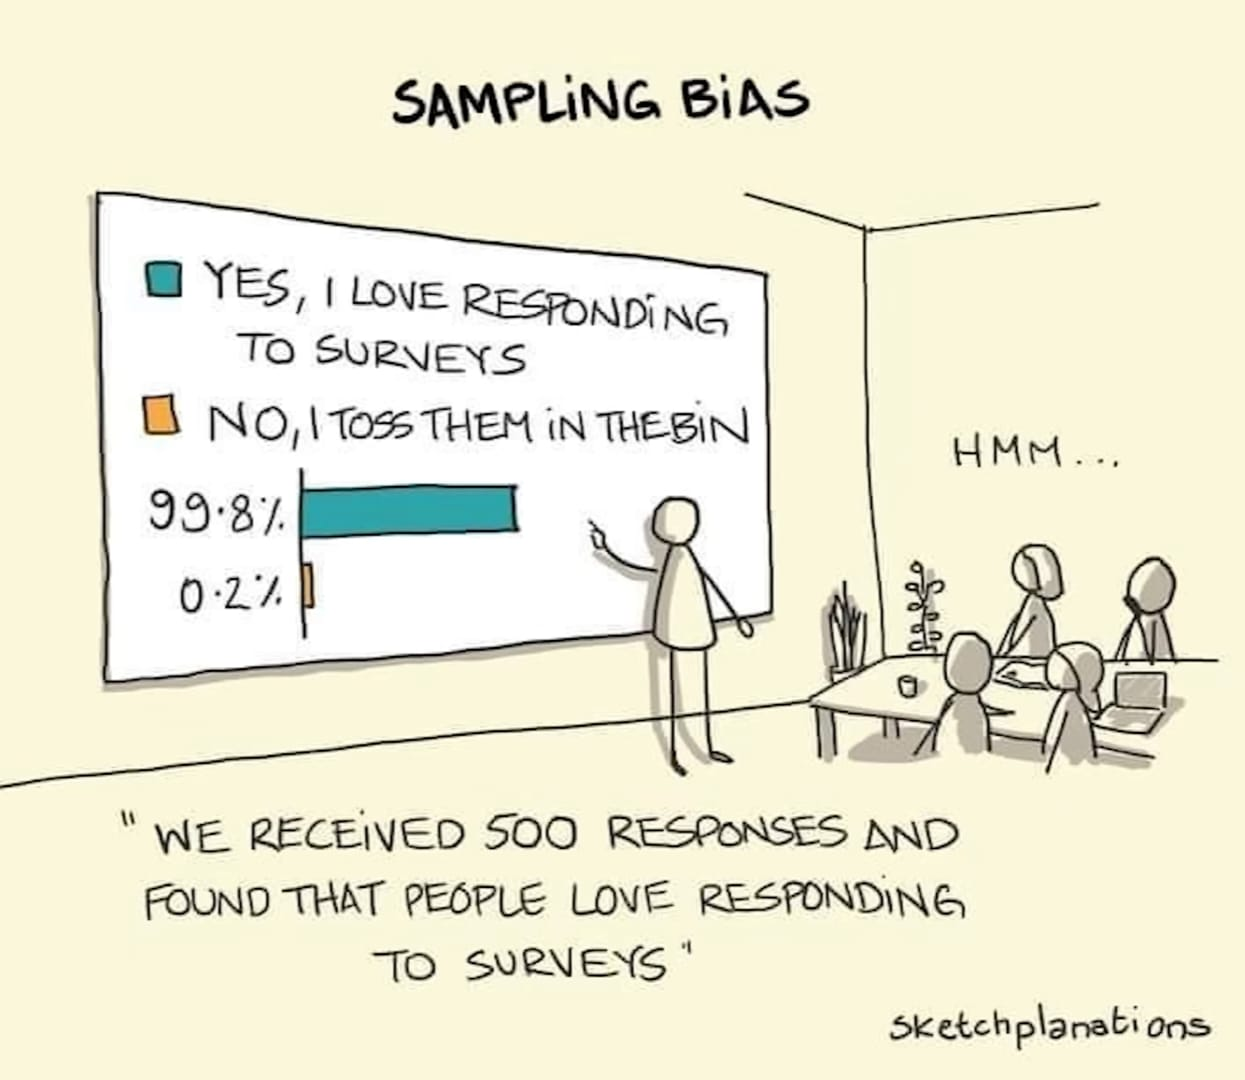
\includegraphics[scale = 0.25]{../images/sampling_bias_meme.jpeg}
    \caption{Example of Sampling Bias}
    \label{Sampling_Bias}
\end{figure}
\newpage
\section{Methodology}
\subsection{Data Collection - Indonesia}
Considering the gigantic dataset pertaining to lip products in Indonesia, secondary data is used in our study in order to minimize time spent collecting the same otherwise. \\

\noindent The initial data for this study was obtained from the sample of 50 lip products given in a prior report \cite{casestudy}. The data given was sourced from 2022 reports, and hence, outdated. We used latest datasets to update 2 parameters - number of shades available in the market and the price of the lipsticks. \\

\noindent To find the latest and credible data, we have used the maximum retail price (MRP) of the product as mentioned on the company's official Indonesian Website. Note that there are some companies which don't have country specific websites (or don't have an operational official website at all). In such cases, we have used Lazada/Shoppee to collect the data. Why these websites? These two websites are leading e-commerce websites in southeast Asia and Taiwan and hence are most credible source that could have been used.

\subsection{Data Collection - India}
The Dataset for Indian Lip Brands was also obtained from secondary sources. Names of all popular Indian makeup brands were noted from various websites \cite{paletteTataCliq} \cite{timesprimeLipsticks2023} \cite{timesprimeMakeupBrands} and also from surveys among students. Then, an exhaustive list of products was prepared for each brand by visiting their official website, sorting all available products on the basis of popularity and noting the top products along with their MRP and number of shades available.
\noindent In some cases where data was missing, we used Amazon and Nykaa to fill in the missing data.


\subsection{Data Analytics}
This study utilizes stratified sampling to determine the sample by dividing the population into subgroups based on factors like brands and product types. Also, the data that is used in this study is nominal in nature since it has categories without necessarily implying mathematical order. Libraries such as matplotlib, numpy, seaborn, and pandas provide easy means to analyze and visualize datasets. \\

\noindent The collected data showed variability in four parameters - Brand, Number of Shades, Type and the Price. Using Stratified Method of Sampling, four tables were made, by counting products grouped by each of the parameters mentioned previously.

\noindent The composition of lip products by type is examined, with details displayed on bar and donut charts. Brand distribution is analyzed using the 'Brand' column, showing the count and percentage of products per brand on a bar plot. \\

\noindent Statistical measures such as mean, median, mode, and quartiles are calculated for prices and the number of shades. Price distribution is visualized through a histogram and box plot, aiding in identifying price ranges and distribution. A bar graph displays the distribution of products based on the number of shades they offer. \\

\noindent Kernel Density Estimation (KDE) is used on histograms to create smooth curves representing the data distribution. This enhances visualization by revealing underlying patterns and providing a refined understanding of price and shade distribution across the dataset. \\

\noindent Color mapping is applied to visualize frequency levels, with lower frequencies represented in blue and higher frequencies in red. Lastly, data is grouped by companies to determine the total number of shades offered by each company, providing insights into shade diversity among different brands.

\newgeometry{left=1cm,right=1cm, top=2cm, bottom=2cm}
\section{Analytics for Indonesia}
\subsection{Raw Data}

\begin{longtable}{lcccc} % Specify the column format here
    \caption{Raw Data for Study (2023) - Indonesia} \label{tab:Table_Raw}                                                                     \\
    \hline
    \textbf{Lip Product}                    & \textbf{Brand}    & \textbf{Type of Lip Product} & \textbf{Shades} & \textbf{Price} \\ \hline
    \endfirsthead
    \multicolumn{5}{c}%
    {{\tablename\ \thetable{} -- Continued from previous page}}                                                                   \\
    \hline
    \textbf{Lip Product}                    & \textbf{Brand}    & \textbf{Type of Lip Product} & \textbf{Shades} & \textbf{Price} \\ \hline
    \endhead
    \hline \multicolumn{5}{r}{{Continued on next page}}                                                                           \\ \hline
    \endfoot
    \hline \hline
    \endlastfoot
    NIVEA LIP BALM SOOTHE \& PRTECT         & Beiersdorf        & Stick                        & 2               & 50000          \\
    Extra lip tint                          & Bobbi Brown       & Stick                        & 10              & 711636         \\
    Perfect Matte Lip Coat                  & Dear Me Beauty    & Liquid                       & 6               & 129000         \\
    Creamytint                              & Emina             & Liquid                       & 5               & 46000          \\
    magic potion lip tint                   & Emina             & Liquid                       & 5               & 50000          \\
    Squeeze me up Lip Matte                 & Emina             & Liquid                       & 4               & 58000          \\
    Smoochies Lip balm                      & Emina             & Solid                        & 1               & 32000          \\
    Matte Lip Liquid                        & ESQA              & Liquid                       & 7               & 165000         \\
    Dear Darling Water gel tint             & Etude House       & Liquid                       & 3               & 55000          \\
    Organic lip balm                        & Eucalie           & Stick                        & 1               & 79000          \\
    lip and cheek dual use liquid           & Focallure         & Liquid                       & 10              & 38000          \\
    Melted Matte Lip                        & Goban Cosmetics   & Liquid                       & 6               & 130000         \\
    Sheen. Tinted lip balm + UV filter      & HALE.             & Stick                        & 4               & 98000          \\
    Urban Lip Cream Matte                   & Implora           & Liquid                       & 20              & 25000          \\
    Beauty Lip \& Cheeck Crayon             & Indoganic         & Crayon                       & 2               & 129000         \\
    Vivid oil tint                          & Innisfree         & Liquid                       & 4               & 104000         \\
    Metallic Lip Cream                      & Inul Beauty       & Liquid                       & 5               & 89000          \\
    Infalible Pro Matte Lip Liquid          & L'oreal           & Liquid                       & 9               & 150000         \\
    Rouge Signature Liquid Matte Lipstick   & L'oreal           & Liquid                       & 14              & 151376         \\
    Color Riche Matte                       & L'oreal           & Stick                        & 8               & 354267         \\
    Intense Matte Lip Cream                 & Liquid            & Liquid                       & 12              & 119000         \\
    Longlasting Matte Lip Cream Metalic     & LT Pro            & Liquid                       & 3               & 109900         \\
    Ultra Light Lip Stain                   & Luxcrime          & Liquid                       & 8               & 79000          \\
    Airy lip mousse                         & Luxcrime          & Liquid                       & 8               & 109000         \\
    Dew tinted 6hr lip moisturizer          & Mad for Makeup    & Stick                        & 6               & 109000         \\
    magnifique lip tint                     & Madame Gie        & Liquid                       & 6               & 33000          \\
    Brilliant Glaze Lip Liquide             & Madame Gie        & Liquid                       & 6               & 35000          \\
    Moist Velvet \& Smooth Lip Liquide      & Madame Gie        & Liquid                       & 6               & 15765          \\
    Hydrastay lip whip                      & Makeover          & Liquid                       & 12              & 119000         \\
    Powestay Transfer Proof Matte Lip Cream & Makeover          & Liquid                       & 12              & 135000         \\
    Sensational Liquid Matte                & Maybelline        & Liquid                       & 19              & 66,023         \\
    color sensational lip tint              & Maybelline        & Liquid                       & 19              & 45000          \\
    Super Stay Matte Ink                    & Maybelline        & Liquid                       & 19              & 239571         \\
    Color sensational the powder mattes     & Maybelline        & Stick                        & 24              & 88900          \\
    Hydra Lip Cheek Tint                    & Mineral Botanica  & Liquid                       & 4               & 51900          \\
    the one A-Z lip balm SPF 25             & Oriflame          & Stick                        & 2               & 149000         \\
    Lip Cream                               & PIXY              & Liquid                       & 16              & 55000          \\
    2 in 1 color tint                       & Purbasari         & Liquid                       & 3               & 51900          \\
    Lip Cream Series                        & Raiku             & Liquid                       & 13              & 118000         \\
    SUEDED! Lip \& Cheek Cream              & Rollover Reaction & Liquid                       & 12              & 109000         \\
    Juicy Lip Balm                          & Rose All day      & Stick                        & 3               & 119000         \\
    Lip Color                               & Runa Beauty       & Stick                        & 5               & 138000         \\
    Lip Care                                & Sensatia Botanica & Liquid                       & 5               & 80000          \\
    Coconut lip sleeping balm               & Tiff Body         & Liquid                       & 1               & 88000          \\
    delight tony tint                       & Tony Moly         & Liquid                       & 3               & 49000          \\
    Exclusive Matte Lip Cream               & Wardah            & Liquid                       & 24              & 66500          \\
    Colorfit Velvet Matte Lip Mousse        & Wardah            & Liquid                       & 14              & 79000          \\
    Everyday Moisture Lip nutrition         & Wardah            & Stick                        & 2               & 28500          \\
    Color Fit Ultralight Matte              & Wardah            & Stick                        & 5               & 47500          \\
    The Simplicity Love You tint            & Y.O.U             & Liquid                       & 4               & 45100          \\
\end{longtable}

\restoregeometry % Restore original page geometry

\newgeometry{top=5.4cm, bottom=5.4cm}
\subsection{Sampled Data}
\subsubsection{On Basis of Brands}

\begin{longtable}{|l|c|c|c|}
    \caption{Products grouped by Brand - Indonesia} \label{tab:prod_by_brand}                                 \\
    \hline
    \textbf{Brand}    & \textbf{Frequency} & \textbf{Percentage} & \textbf{Cumulative Percentage} \\ \hline
    \endfirsthead
    \multicolumn{4}{c}%
    {{\tablename\ \thetable{} -- Continued from previous page}}                                   \\
    \hline
    \textbf{Brand}    & \textbf{Frequency} & \textbf{Percentage} & \textbf{Cumulative Percentage} \\ \hline
    \endhead
    \hline \multicolumn{4}{r}{{Continued on next page}}                                           \\ \hline
    \endfoot
    \hline \hline
    \endlastfoot
    Beiersdorf        & 1                  & 2.0                 & 2.0                            \\
    Bobbi Brown       & 1                  & 2.0                 & 4.0                            \\
    Dear Me Beauty    & 1                  & 2.0                 & 6.0                            \\
    Emina             & 4                  & 8.0                 & 14.0                           \\
    ESQA              & 1                  & 2.0                 & 16.0                           \\
    Etude House       & 1                  & 2.0                 & 18.0                           \\
    Eucalie           & 1                  & 2.0                 & 20.0                           \\
    Focallure         & 1                  & 2.0                 & 22.0                           \\
    Goban Cosmetics   & 1                  & 2.0                 & 24.0                           \\
    HALE.             & 1                  & 2.0                 & 26.0                           \\
    Implora           & 1                  & 2.0                 & 28.0                           \\
    Indoganic         & 1                  & 2.0                 & 30.0                           \\
    Innisfree         & 1                  & 2.0                 & 32.0                           \\
    Inul Beauty       & 1                  & 2.0                 & 34.0                           \\
    L'oreal           & 3                  & 6.0                 & 40.0                           \\
    Liquid            & 1                  & 2.0                 & 42.0                           \\
    LT Pro            & 1                  & 2.0                 & 44.0                           \\
    Luxcrime          & 2                  & 4.0                 & 48.0                           \\
    Mad for Makeup    & 1                  & 2.0                 & 50.0                           \\
    Madame Gie        & 3                  & 6.0                 & 56.0                           \\
    Makeover          & 2                  & 4.0                 & 60.0                           \\
    Maybelline        & 4                  & 8.0                 & 68.0                           \\
    Mineral Botanica  & 1                  & 2.0                 & 70.0                           \\
    Oriflame          & 1                  & 2.0                 & 72.0                           \\
    PIXY              & 1                  & 2.0                 & 74.0                           \\
    Purbasari         & 1                  & 2.0                 & 76.0                           \\
    Raiku             & 1                  & 2.0                 & 78.0                           \\
    Rollover Reaction & 1                  & 2.0                 & 80.0                           \\
    Rose All day      & 1                  & 2.0                 & 82.0                           \\
    Runa Beauty       & 1                  & 2.0                 & 84.0                           \\
    Sensatia Botanica & 1                  & 2.0                 & 86.0                           \\
    Tiff Body         & 1                  & 2.0                 & 88.0                           \\
    Tony Moly         & 1                  & 2.0                 & 90.0                           \\
    Wardah            & 4                  & 8.0                 & 98.0                           \\
    Y.O.U             & 1                  & 2.0                 & 100.0                          \\
\end{longtable}
\newpage
\subsubsection{On Basis of Type}
\begin{longtable}{|l|c|c|c|} % Specify the column format here
    \caption{Products grouped by Type - Indonesia} \label{tab:change_label_here}                          \\
    \hline
    \textbf{Type} & \textbf{Frequency} & \textbf{Percentage} & \textbf{Cumulative Percentage} \\ \hline
    \endfirsthead
    \multicolumn{4}{c}%
    {{\tablename\ \thetable{} -- Continued from previous page}}                               \\
    \hline
    \textbf{Type} & \textbf{Frequency} & \textbf{Percentage} & \textbf{Cumulative Percentage} \\ \hline
    \endhead
    \hline \multicolumn{4}{r}{{Continued on next page}}                                       \\ \hline
    \endfoot
    \hline \hline
    \endlastfoot
    Stick         & 12                 & 24.0                & 24.0                           \\
    Liquid        & 36                 & 72.0                & 96.0                           \\
    Solid         & 1                  & 2.0                 & 98.0                           \\
    Crayon        & 1                  & 2.0                 & 100.0                          \\
\end{longtable}
\subsubsection{On Basis of Shades}
\begin{longtable}{|c|c|c|c|} % Specify the column format here
    \caption{Products grouped by Shades - Indonesia} \label{tab:prod_by_shades}                             \\
    \hline
    \textbf{Shades} & \textbf{Frequency} & \textbf{Percentage} & \textbf{Cumulative Percentage} \\ \hline
    \endfirsthead
    \multicolumn{4}{c}%
    {{\tablename\ \thetable{} -- Continued from previous page}}                                 \\
    \hline
    \textbf{Shades} & \textbf{Frequency} & \textbf{Percentage} & \textbf{Cumulative Percentage} \\ \hline
    \endhead
    \hline \multicolumn{4}{r}{{Continued on next page}}                                         \\ \hline
    \endfoot
    \hline \hline
    \endlastfoot
    1               & 3                  & 6.0                 & 6.0                            \\
    2               & 4                  & 8.0                 & 14.0                           \\
    3               & 5                  & 10.0                & 24.0                           \\
    4               & 5                  & 10.0                & 34.0                           \\
    5               & 6                  & 12.0                & 46.0                           \\
    6               & 6                  & 12.0                & 58.0                           \\
    7               & 1                  & 2.0                 & 60.0                           \\
    8               & 3                  & 6.0                 & 66.0                           \\
    9               & 1                  & 2.0                 & 68.0                           \\
    10              & 2                  & 4.0                 & 72.0                           \\
    12              & 4                  & 8.0                 & 80.0                           \\
    13              & 1                  & 2.0                 & 82.0                           \\
    14              & 2                  & 4.0                 & 86.0                           \\
    16              & 1                  & 2.0                 & 88.0                           \\
    19              & 3                  & 6.0                 & 94.0                           \\
    20              & 1                  & 2.0                 & 96.0                           \\
    24              & 2                  & 4.0                 & 100.0                          \\
\end{longtable}
\restoregeometry

\newgeometry{top=3cm, bottom=3cm}
\subsection{Graphs and Stats}
\begin{center}
    \begin{longtable}{|>{\columncolor{gray!15}}l|l|l|} % Adjust the number of columns and alignment as needed
        \caption{Descriptive Statistics of Shades and Prices - Indonesia} \label{tab:statistics} \\
        \hline
        \rowcolor{gray!50}
        \textbf{Attribute}     & \textbf{Shades} & \textbf{Price}                    \\ \hline
        \endfirsthead
        \multicolumn{3}{c}%
        {{\tablename\ \thetable{} -- Continued from previous page}}                  \\
        \hline
        \textbf{Attribute}     & \textbf{Shades} & \textbf{Price}                    \\ \hline
        \endhead
        \hline \multicolumn{3}{r}{{Continued on next page}}                          \\ \hline
        \endfoot
        \hline \hline
        \endlastfoot
        Count                  & 50              & 50                                \\
        Mean                   & 8.04            & 104456.76                         \\
        Median                 & 6               & 84000                             \\
        Mode                   & 5, 6            & 79000, 109000, 119000             \\
        Std Dev                & 6.11            & 105480.23                         \\
        Variance               & 37.3            & 11126079540.23                    \\
        Minimum                & 1               & 15765                             \\
        Maximum                & 24              & 711636                            \\
        \hline
        \rowcolor{gray!50}
        \textbf{Percentiles}:  &                 &                                   \\ \hline
        \hspace{0.3cm} - 0th   & 1               & 15765                             \\
        \hspace{0.3cm} - 25th  & 4               & 50000                             \\
        \hspace{0.3cm} - 50th  & 6               & 84000                             \\
        \hspace{0.3cm} - 75th  & 12              & 119000                            \\
        \hspace{0.3cm} - 100th & 24              & 711636                            \\
    \end{longtable}

    \begin{figure}[htbp]
        \centering
        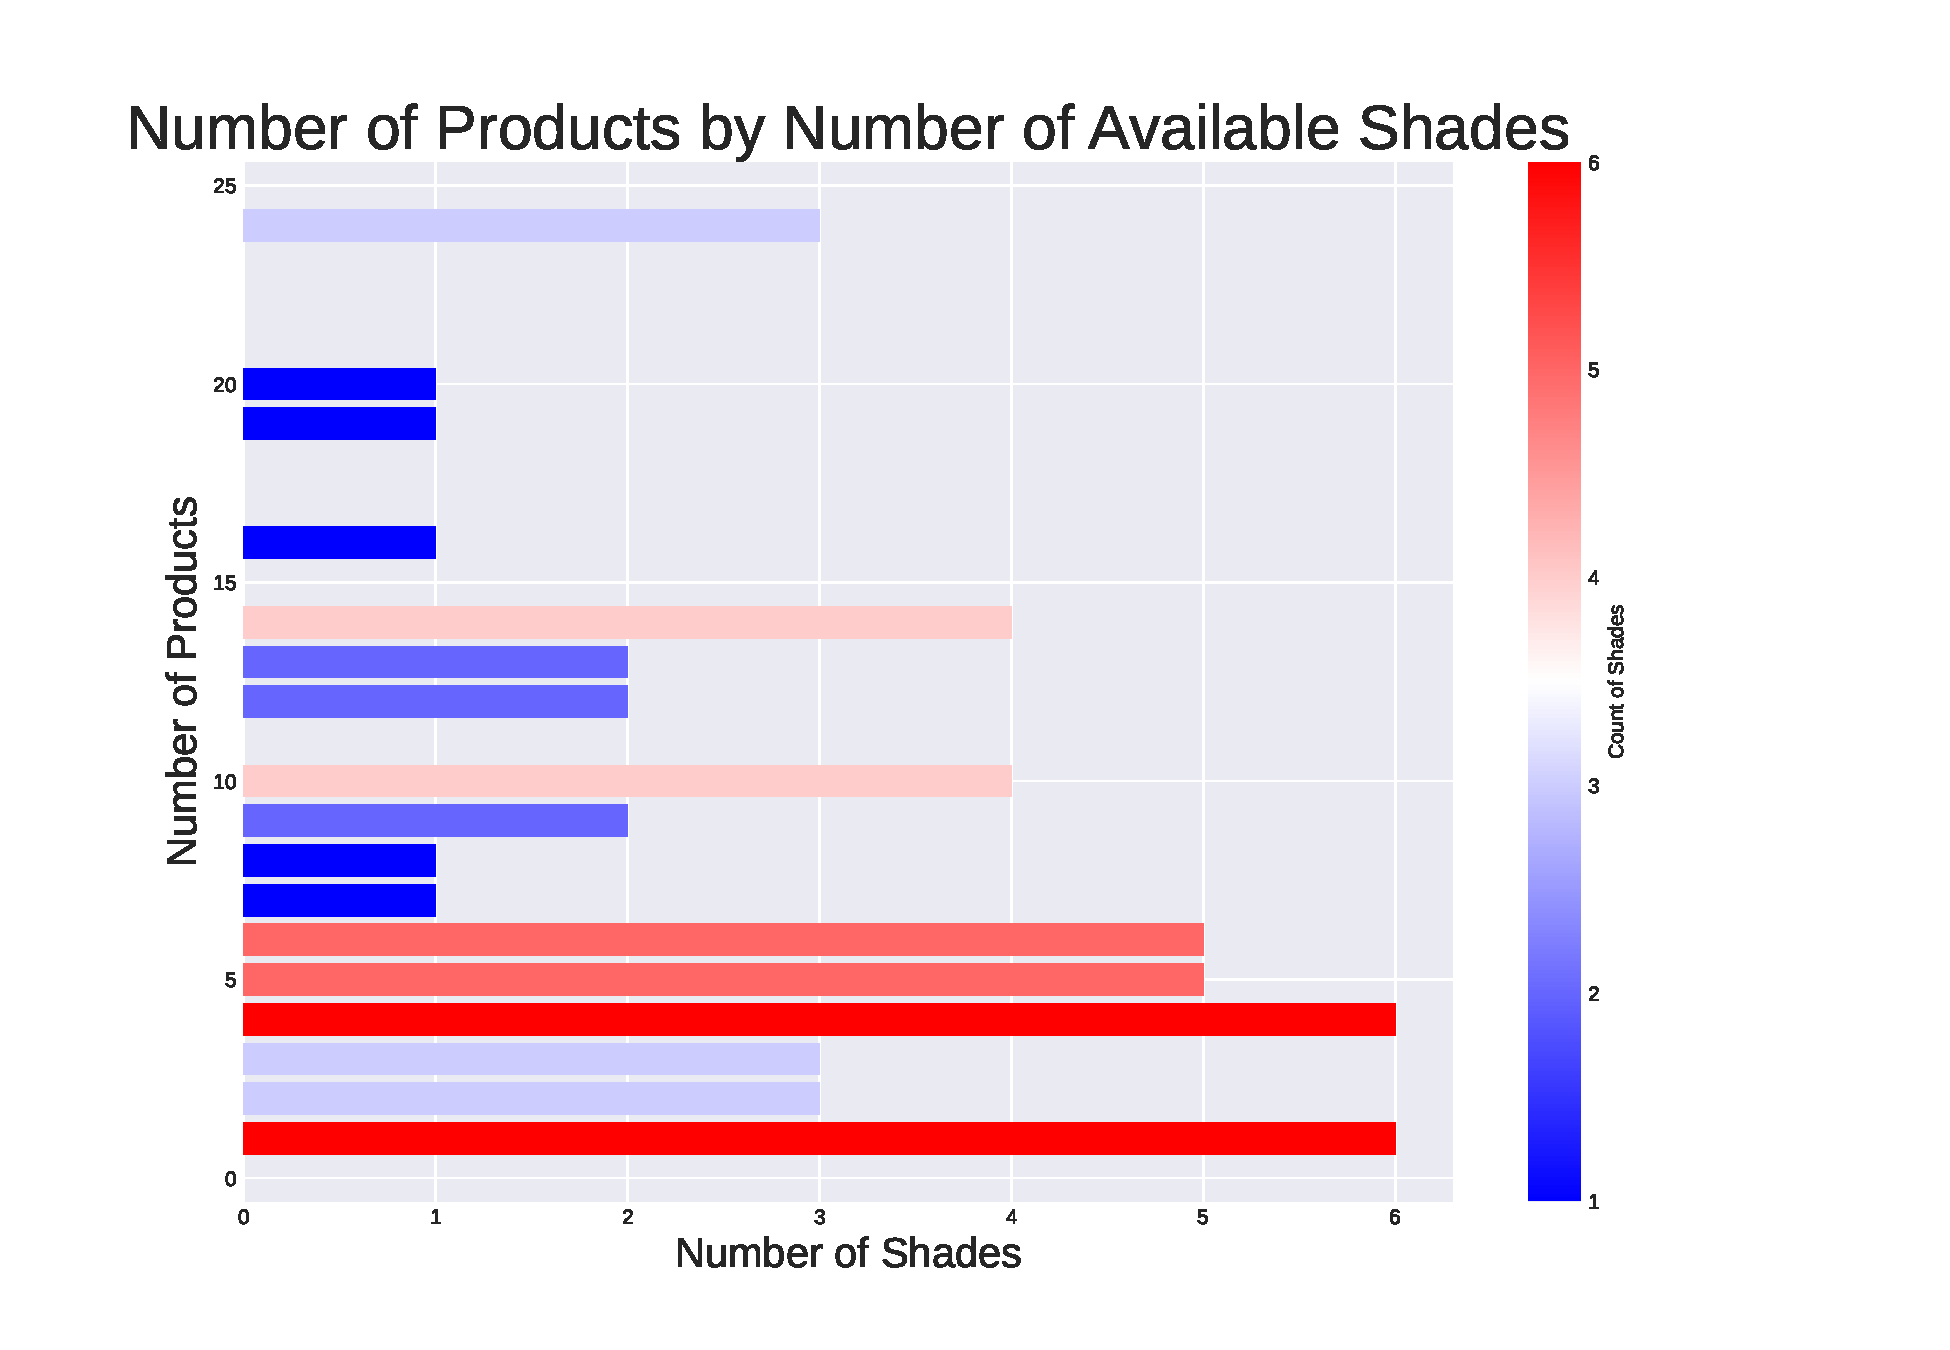
\includegraphics[scale=0.4]{../images/Indonesia-graphs/TotalProductsByShades.pdf}
        \caption{Total Products Grouped by Shades - Indonesia}
        \label{Products_by_Shades}
    \end{figure}

    \newgeometry{left=2cm,right=2cm, top=1cm, bottom=1.5cm}

    \begin{landscape}
        \begin{figure}[htbp]
            \centering
            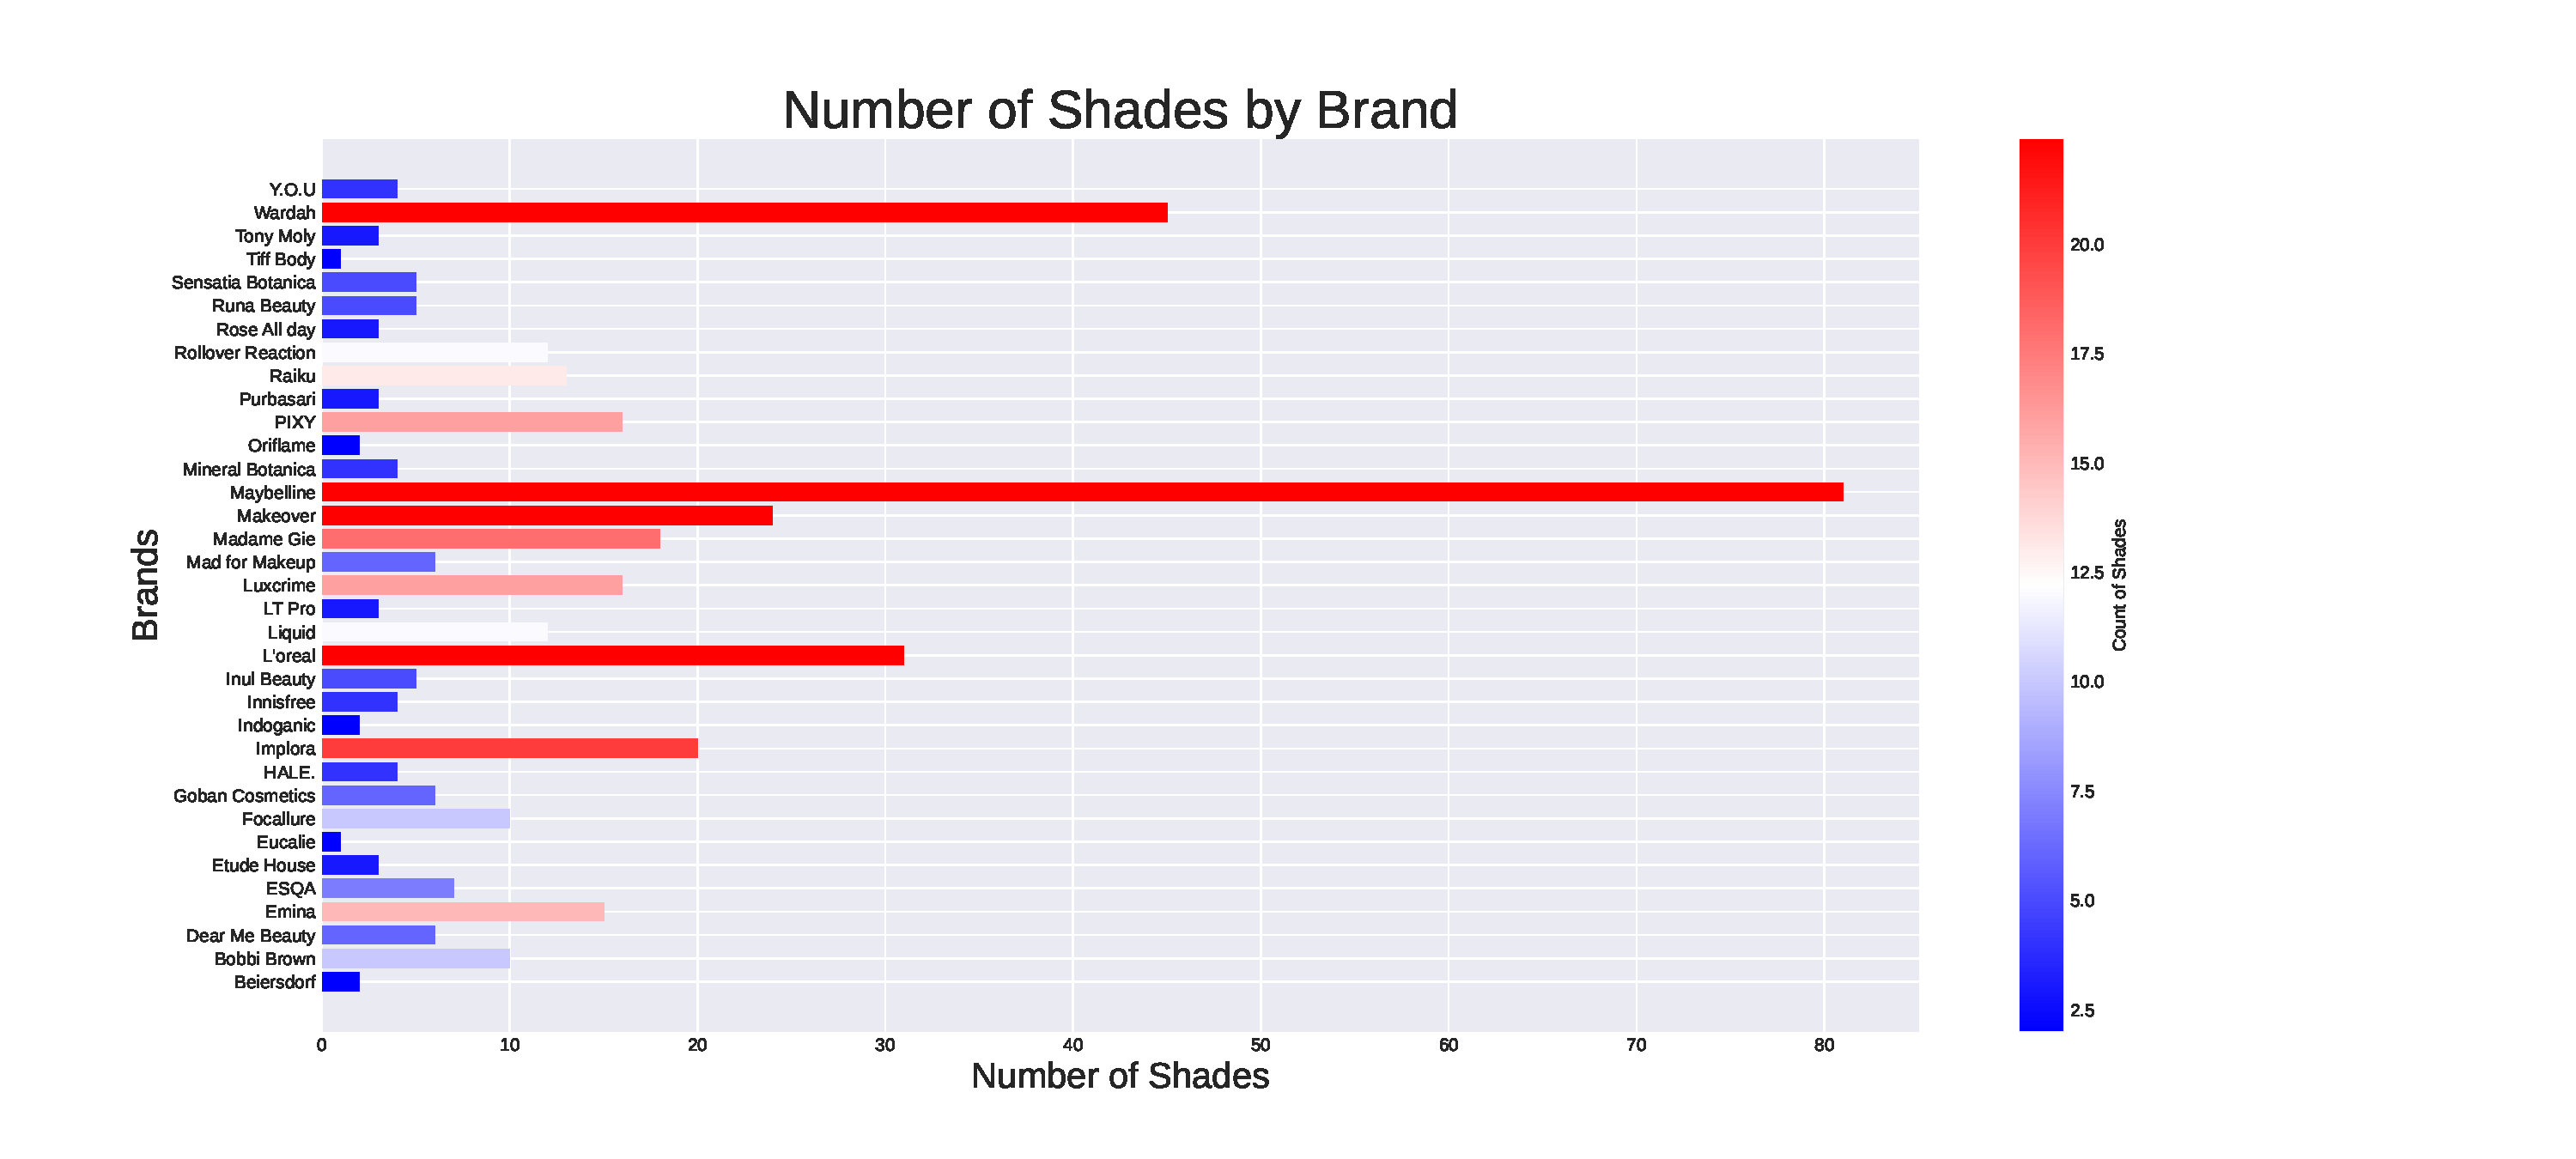
\includegraphics[scale=0.55]{../images/Indonesia-graphs/TotalShadesByBrand.pdf}
            \caption{Total Shades Grouped by Brands - Indonesia}
            \label{Shades_by_Brands}
        \end{figure}
    \end{landscape}

    \begin{landscape}
        \begin{figure}[htbp]
            \centering
            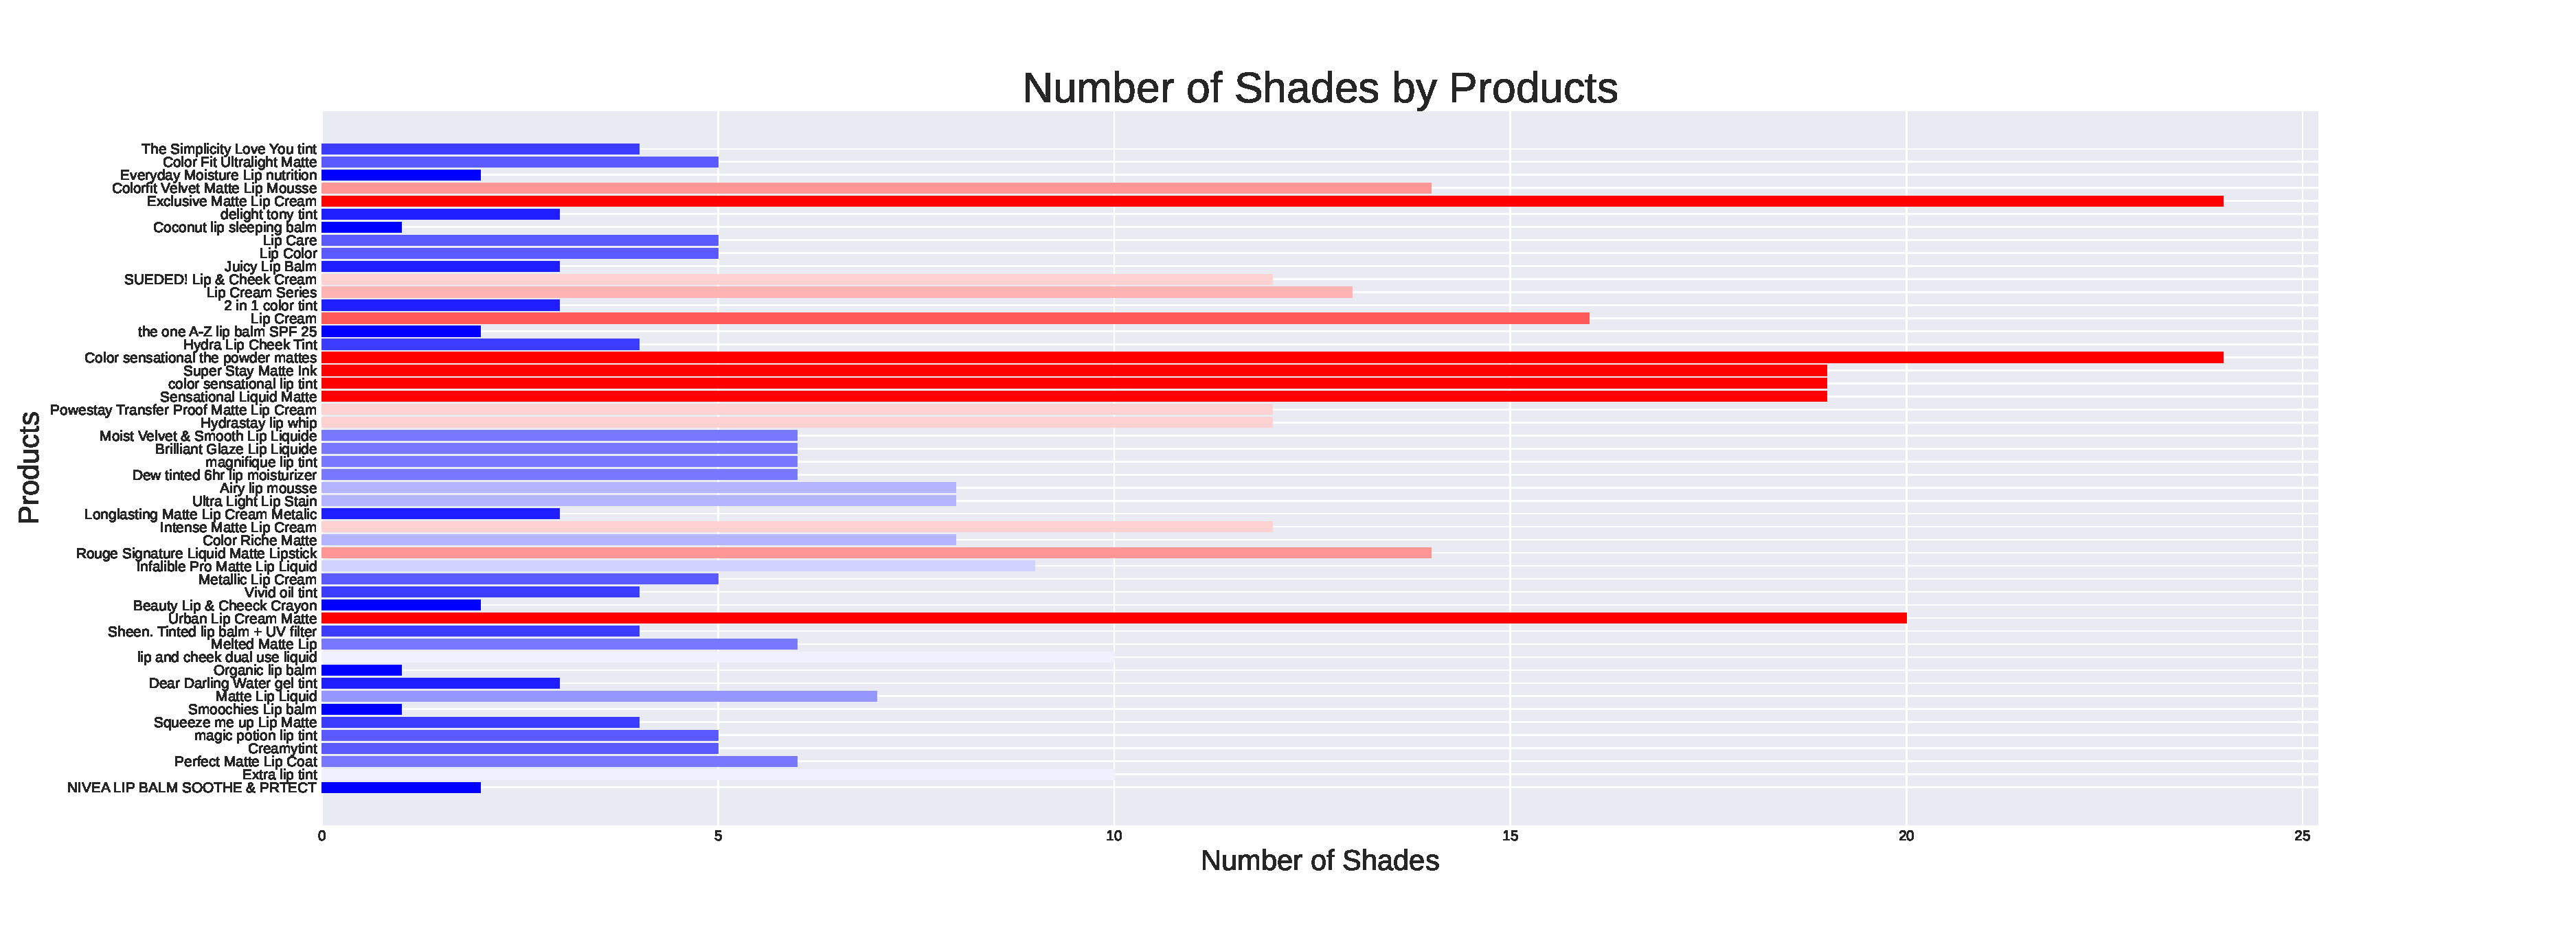
\includegraphics[scale=0.49]{../images/Indonesia-graphs/TotalShadesByProduct.pdf}
            \caption{Total Shades Grouped by Product - Indonesia}
            \label{Shades_by_Product}
        \end{figure}
    \end{landscape}

    \begin{figure}[htbp]
        \centering
        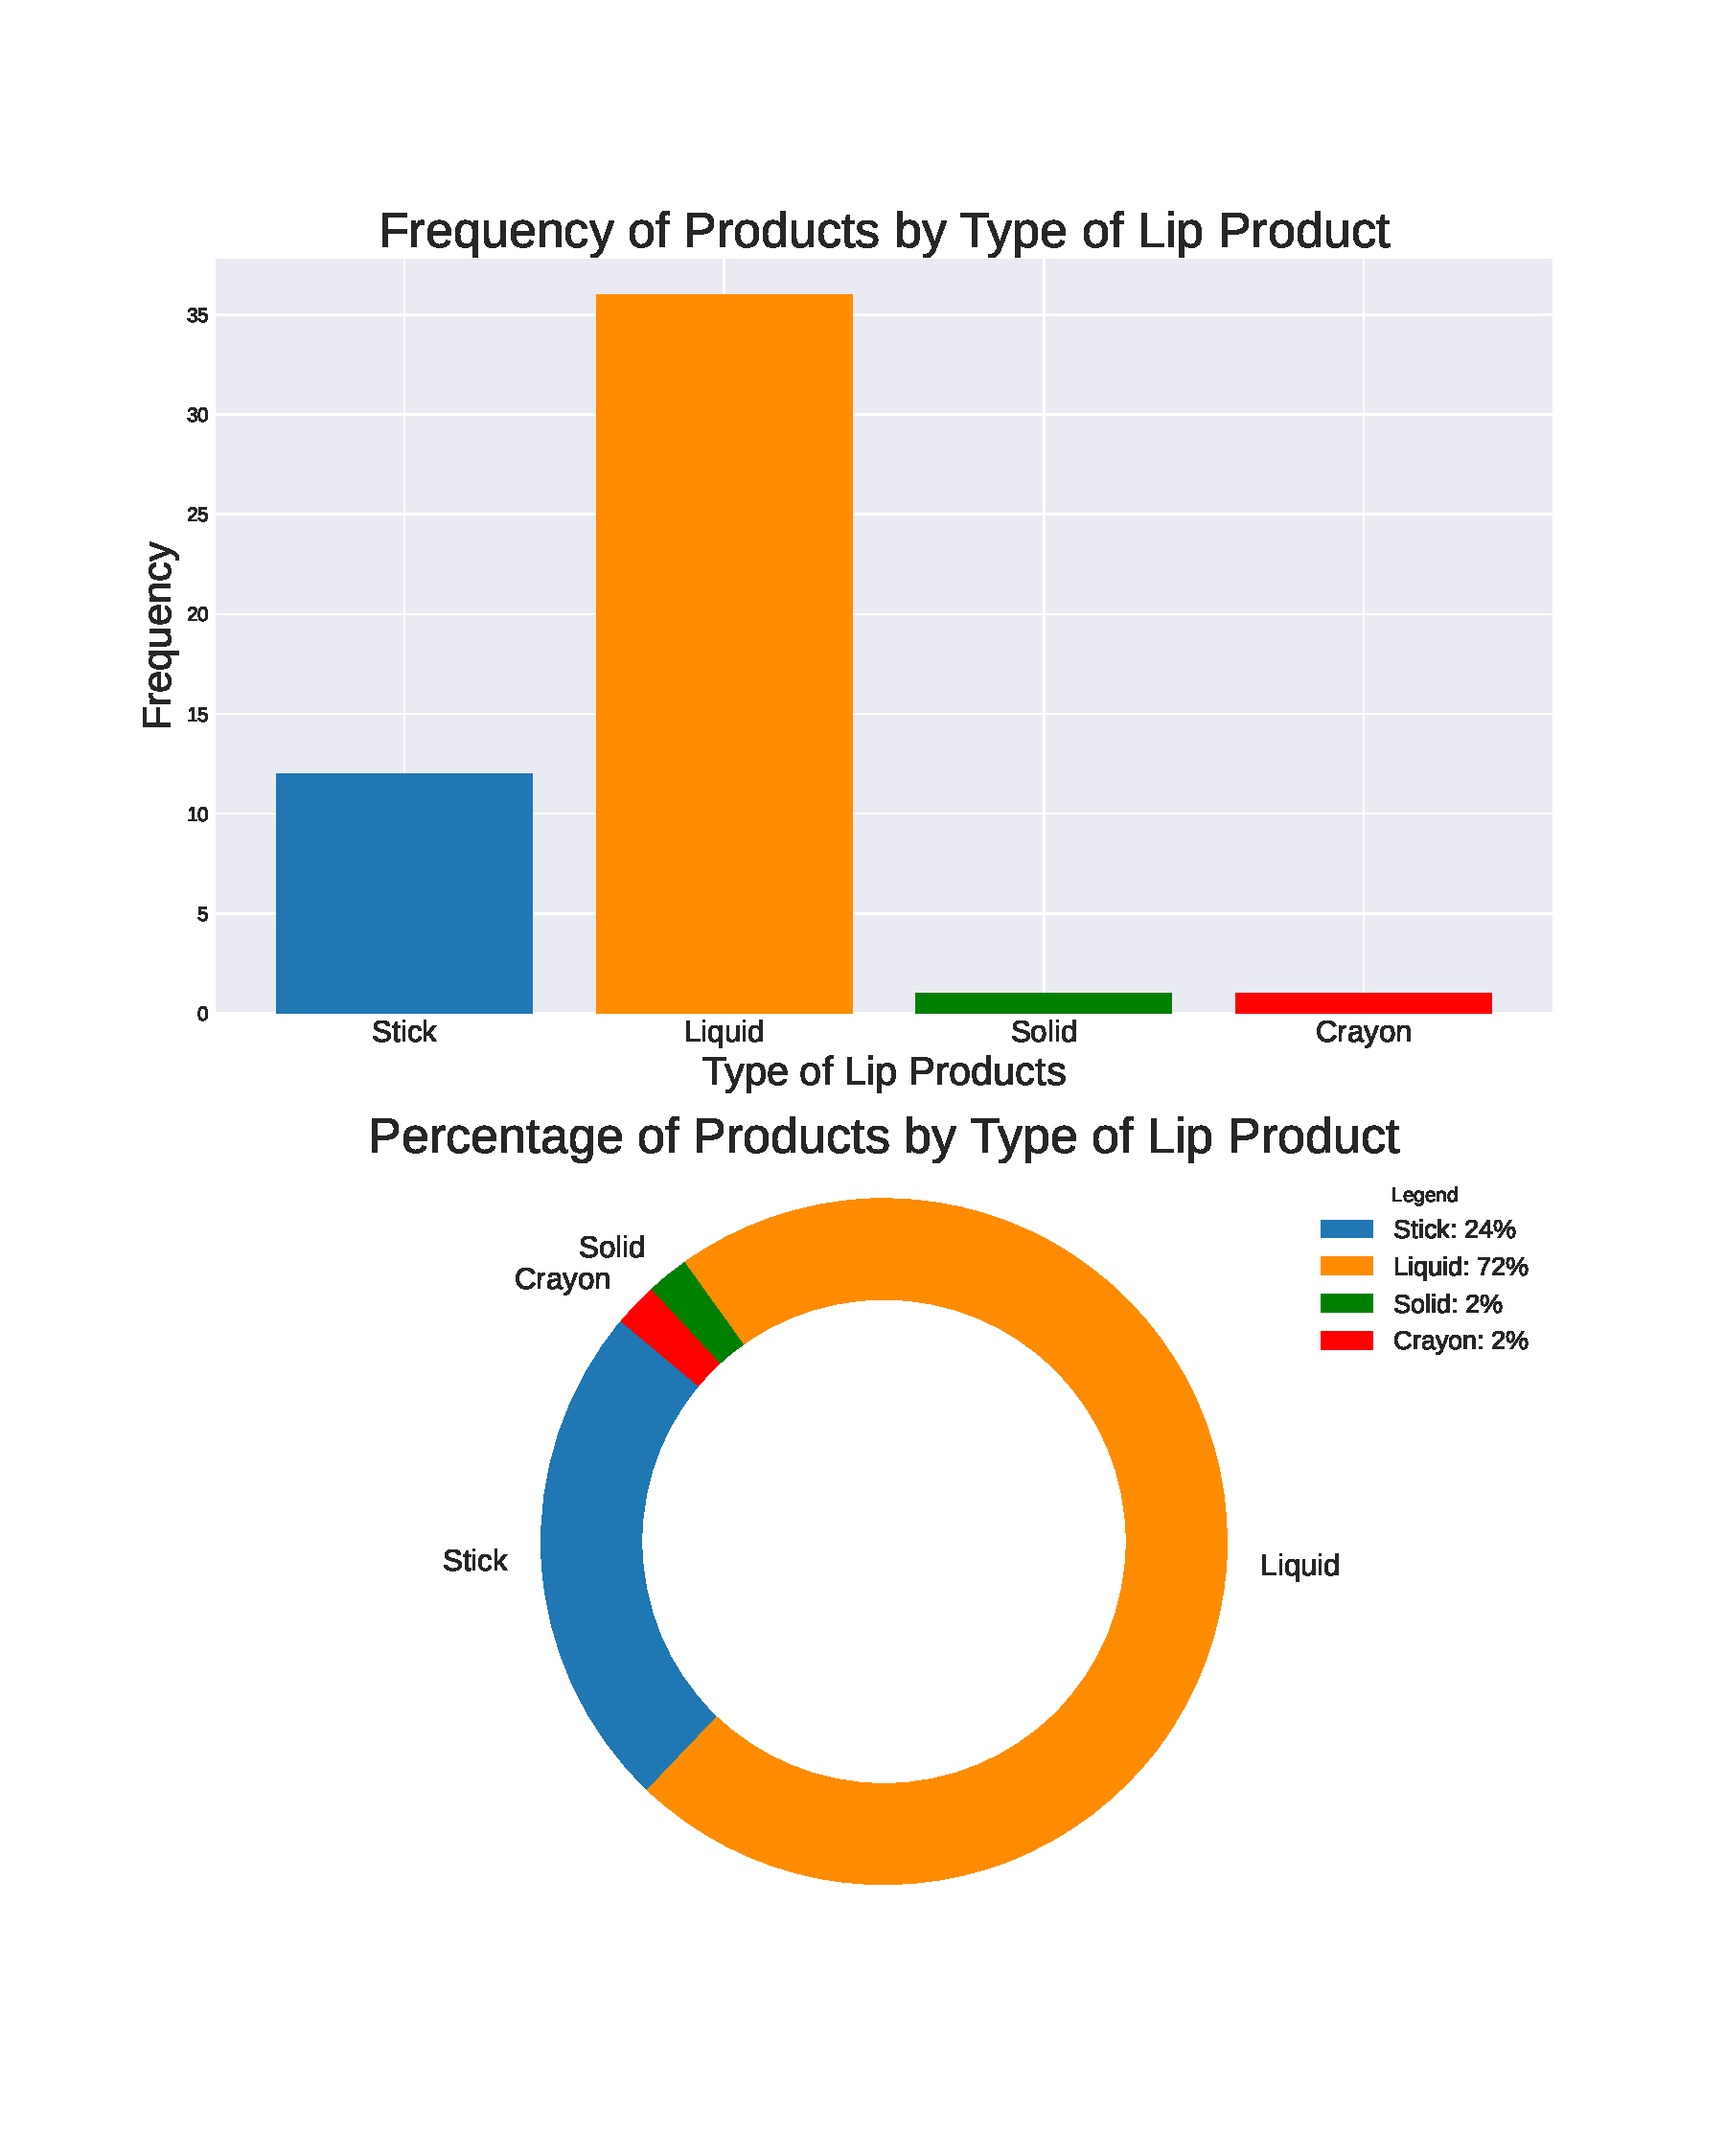
\includegraphics[scale=0.6]{../images/Indonesia-graphs/TotalProductsbyType.pdf}
        \caption{Total Products Grouped by Type - Indonesia}
        \label{Products_by_Type}
    \end{figure}

    \begin{figure}[htbp]
        \centering
        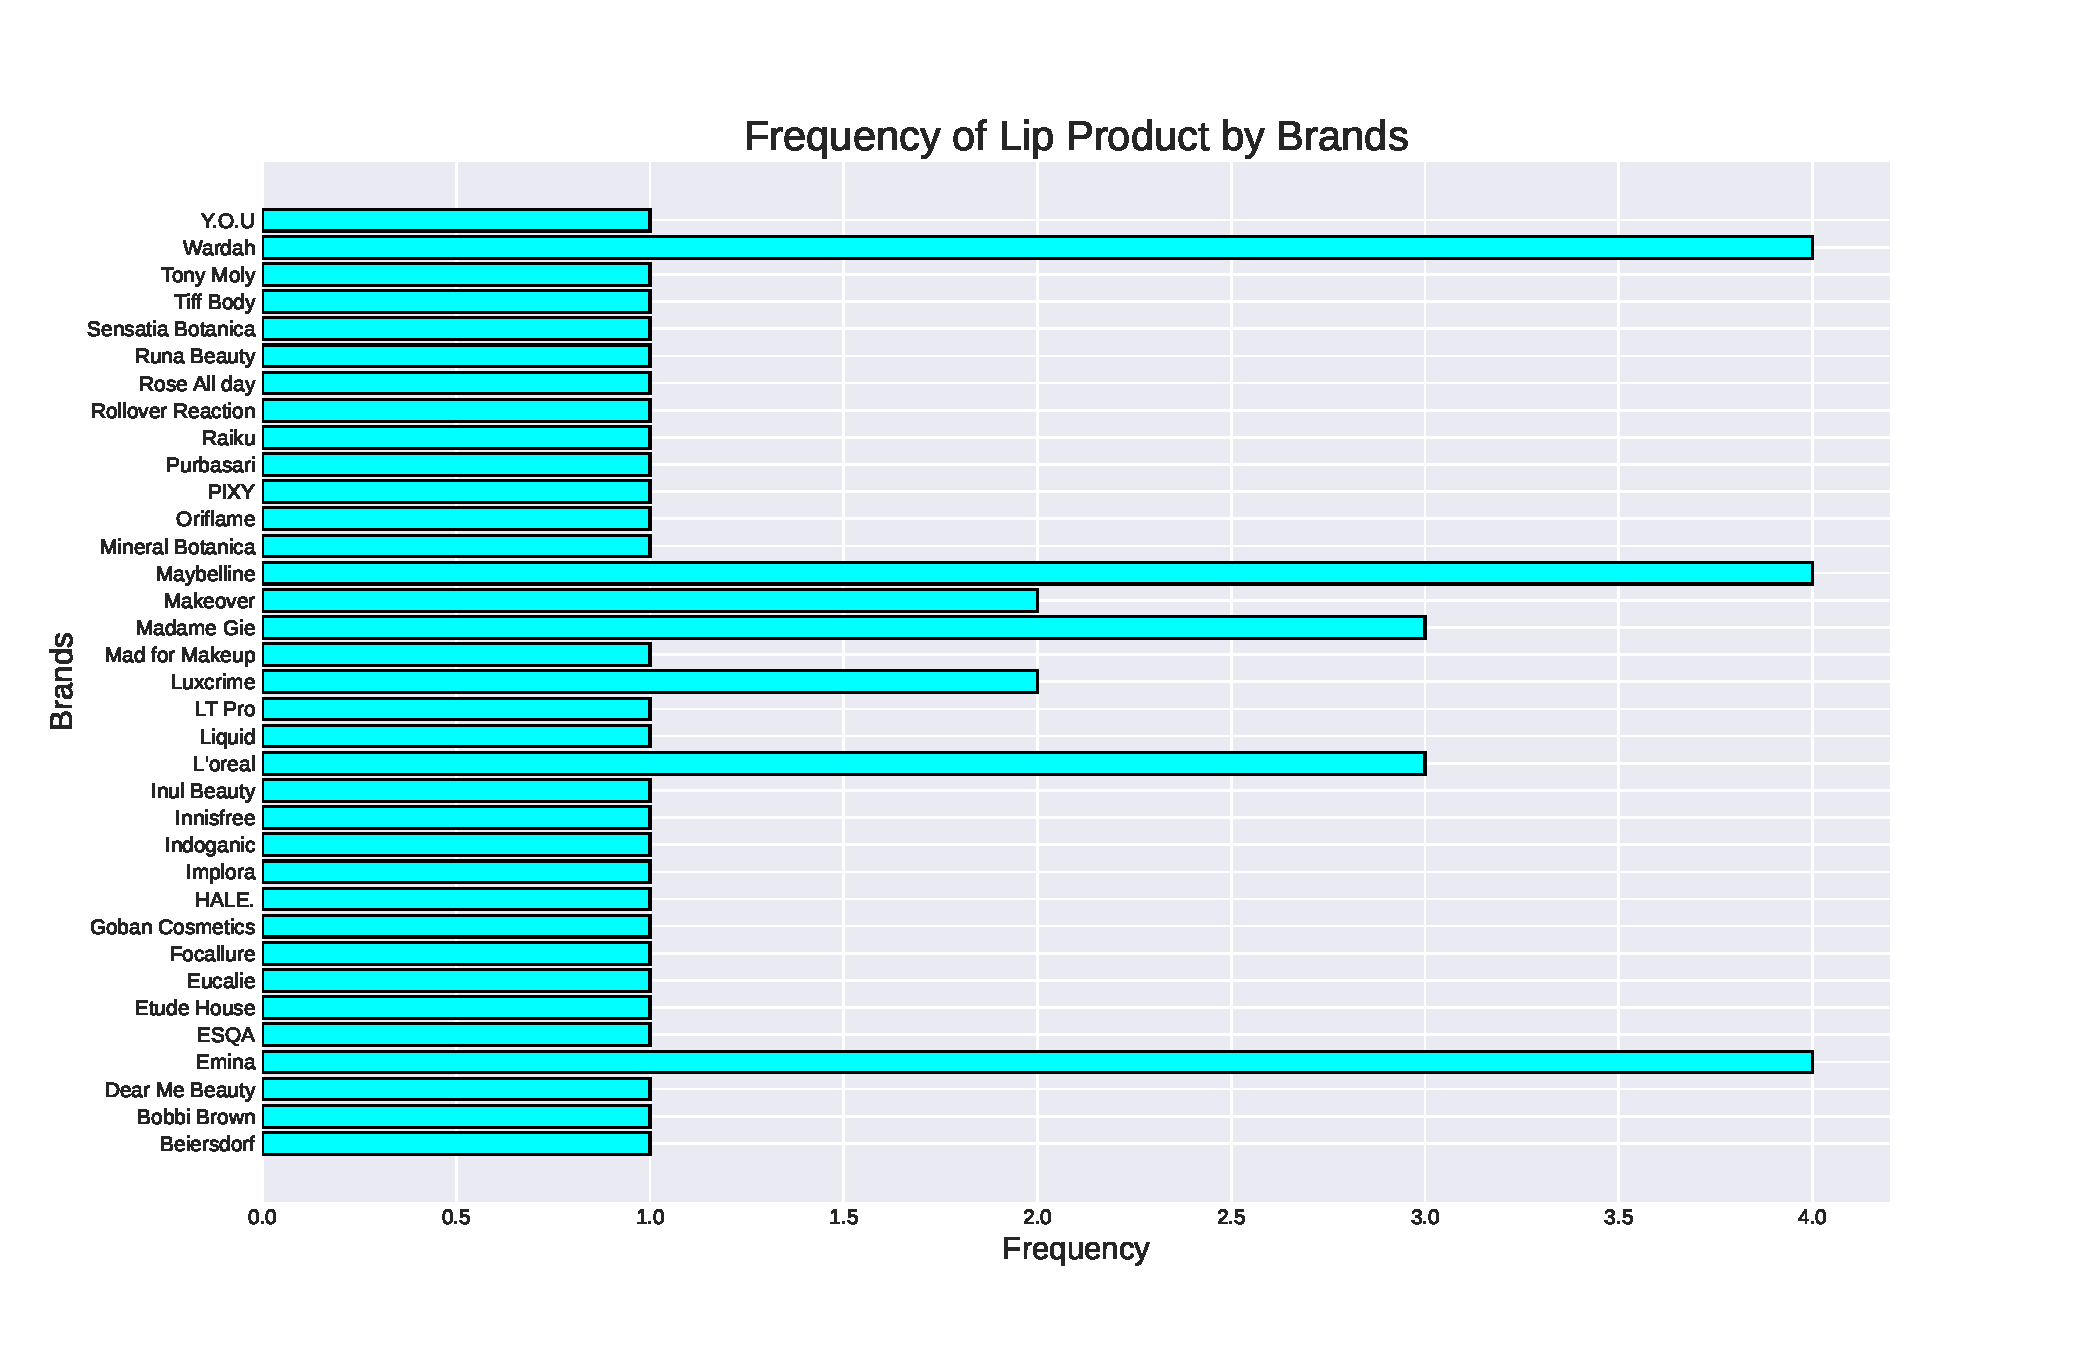
\includegraphics[scale=0.5]{../images/Indonesia-graphs/Brand_Frequency.pdf}
        \caption{Frequency of Products by Brands - Indonesia}
        \label{Products_by_Brands}
    \end{figure}

    \begin{figure}[htbp]
        \centering
        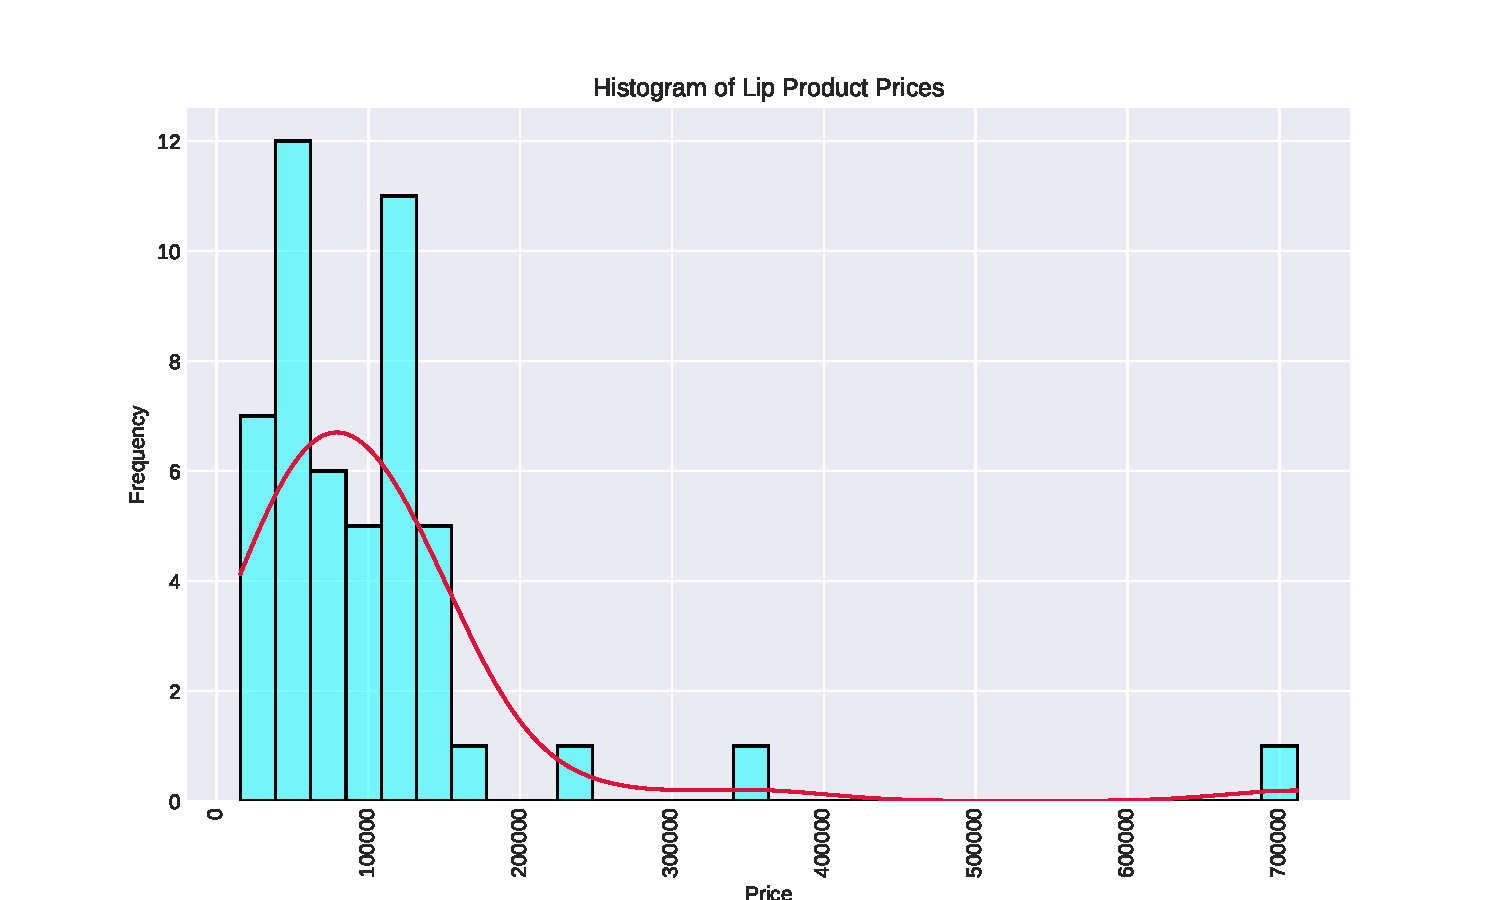
\includegraphics[scale=0.6]{../images/Indonesia-graphs/KDE_Prices.pdf}
        \caption{Product - Price Distribution - with KDE - Indonesia}
        \label{KDE_Prices}
    \end{figure}

    \begin{figure}[htbp]
        \centering
        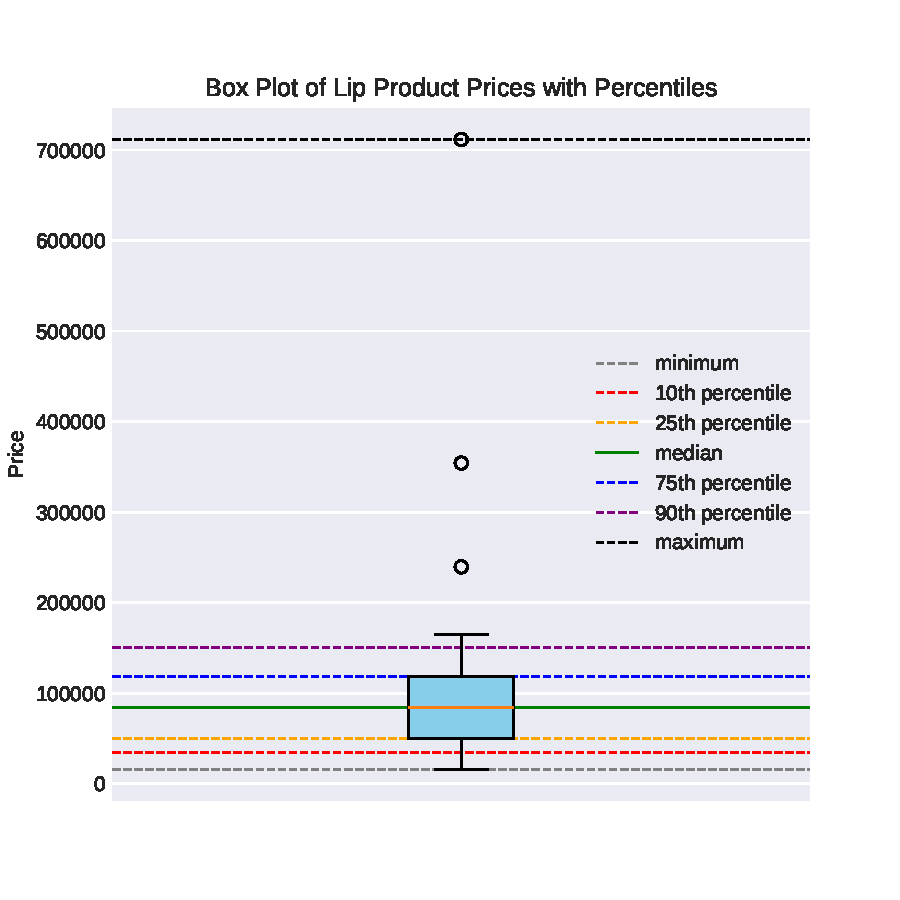
\includegraphics[scale=0.6]{../images/Indonesia-graphs/Box_Prices.pdf}
        \caption{Product - Price Distribution - BoxPlot - Indonesia}
        \label{Box_Prices}
    \end{figure}

    \begin{figure}[htbp]
        \centering
        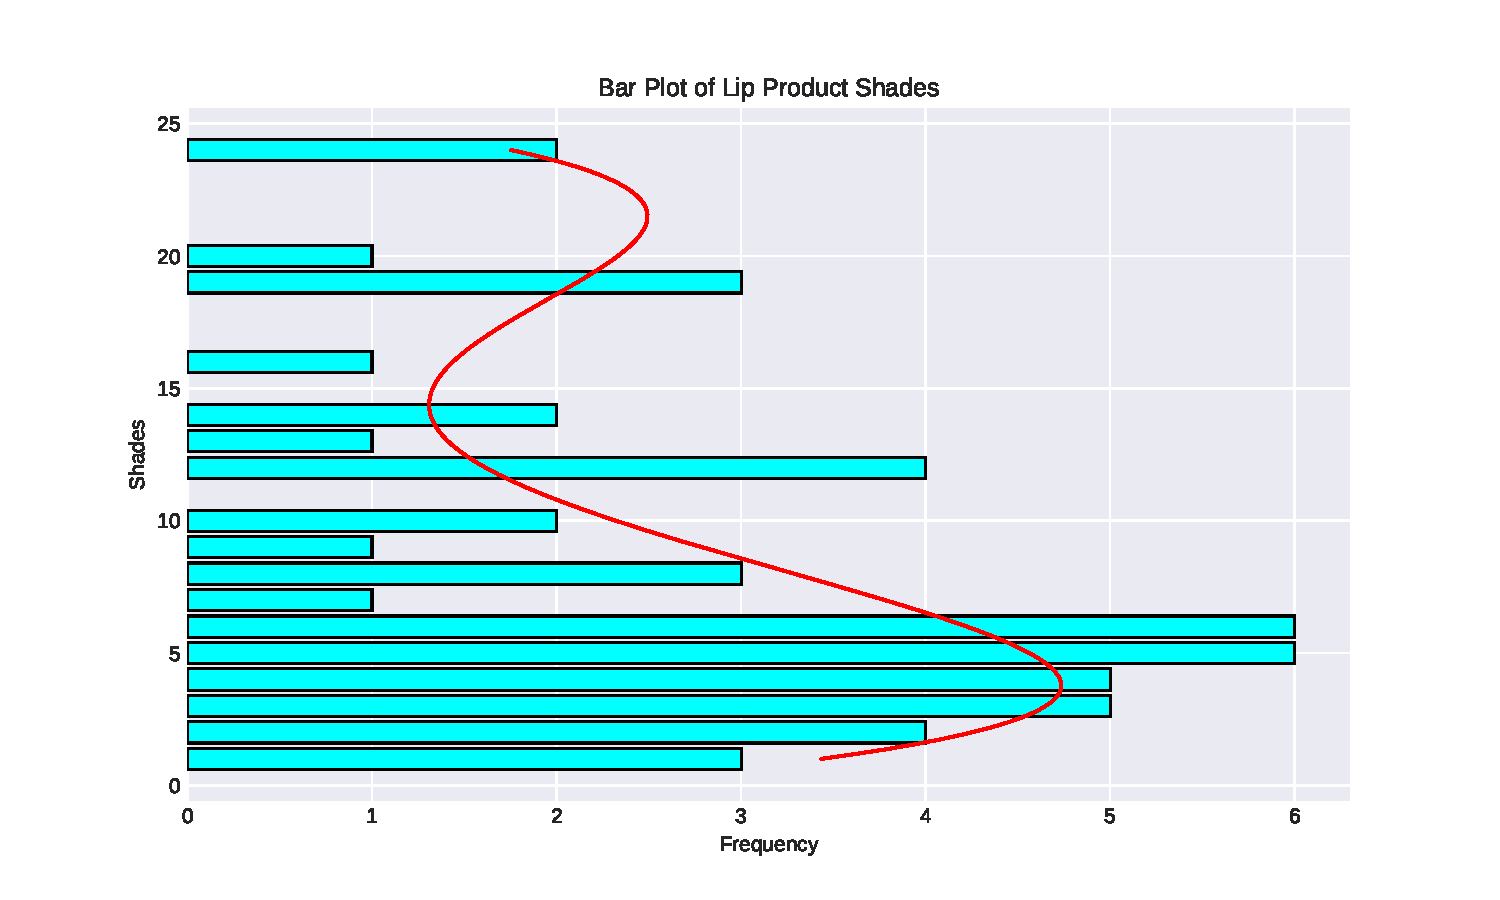
\includegraphics[scale=0.6]{../images/Indonesia-graphs/KDE_Shades.pdf}
        \caption{Product - Shades Distribution - with KDE - Indonesia}
        \label{KDE_Shades}
    \end{figure}
    \restoregeometry

\end{center}
\restoregeometry



\newgeometry{left=2.3cm,right=2.3cm, top=5.4cm, bottom=5.4cm}
\section{Analytics for India}
\subsection{Raw Data}

\begin{longtable}{lcccc} % Specify the column format here
    \caption{Raw Data for Study (2023) - India} \label{tab:Table_Raw_ind}                                                              \\
    \hline
    \textbf{Lip Product}                                & \textbf{Brand}  & \textbf{Type}   & \textbf{Shades} & \textbf{Price} \\ \hline
    \endfirsthead
    \multicolumn{5}{c}%
    {{\tablename\ \thetable{} -- Continued from previous page}}                                                                \\
    \hline
    \textbf{Lip Product}                                & \textbf{Brand}  & \textbf{Type}   & \textbf{Shades} & \textbf{Price} \\ \hline
    \endhead
    \hline \multicolumn{5}{r}{{Continued on next page}}                                                                        \\ \hline
    \endfoot
    \hline \hline
    \endlastfoot
    Color Sensational Creamy Matte Lipstick             & Maybelline      & Lipstick        & 44              & 299            \\
    SuperStay Matte Ink Liquid Lipstick                 & Maybelline      & Liquid Lipstick & 30              & 699            \\
    SuperStay Matte Ink Crayon Lipstick                 & Maybelline      & Lip Crayon      & 10              & 599            \\
    Lifter Gloss                                        & Maybelline      & Lip Gloss       & 4               & 799            \\
    Baby Lips Loves Color Lip Balm                      & Maybelline      & Lip Balm        & 3               & 175            \\
    Baby Lips Bloom Lip Balm                            & Maybelline      & Lip Balm        & 2               & 180            \\
    9 to 5 Powerplay Priming Matte Lip Color            & Lakmé           & Lipstick        & 35              & 599            \\
    Absolute Matte Melt Liquid Lip Color                & Lakmé           & Liquid Lipstick & 15              & 800            \\
    Absolute Plump and Shine Lip Gloss                  & Lakmé           & Lip Gloss       & 8               & 800            \\
    Lip Love Chapstick                                  & Lakmé           & Lip Balm        & 7               & 160            \\
    Xtraordin-airy Lip Mousse                           & Lakmé           & Liquid Lipstick & 14              & 700            \\
    Color Riche Lipstick                                & L'Oréal Paris   & Lipstick        & 43              & 799            \\
    Rouge Signature Matte Liquid Lipstick               & L'Oréal Paris   & Liquid Lipstick & 13              & 899            \\
    Matte Luxe Lipstick                                 & Nykaa           & Lipstick        & 12              & 849            \\
    So Matte Lipstick                                   & Nykaa           & Lipstick        & 48              & 450            \\
    So Creme! Creamy Matte Lipstick                     & Nykaa           & Lipstick        & 18              & 329            \\
    Matte To Last! Liquid Lipstick                      & Nykaa           & Liquid Lipstick & 24              & 675            \\
    Gloss It Up! High Shine Lip Gloss                   & Nykaa           & Lip Gloss       & 4               & 550            \\
    Macaron Lip Balm                                    & Nykaa           & Lip Balm        & 7               & 299            \\
    Lips Don't Lie! Line \& Fill Lip Liner              & Nykaa           & Lip Liner       & 16              & 399            \\
    Ultra Matte Lipstick                                & Nykaa           & Lipstick        & 17              & 649            \\
    Matte-ilicious lip crayon lipstick                  & Nykaa           & Lip Crayon      & 8               & 799            \\
    Serial Kisser Moisturising Tinted Lip Balm          & Nykaa           & Lip Balm        & 5               & 179            \\
    Paintstix! Waterproof Matte Lipstick                & Nykaa           & Lipstick        & 9               & 525            \\
    All day matte liquid lipstick                       & Nykaa           & Liquid Lipstick & 19              & 399            \\
    Gloss it up pH Lip gloss oil                        & Nykaa           & Lip gloss       & 1               & 575            \\
    Get set matte! Demi matte lip cream liquid lipstick & Nykaa           & Liquid Lipstick & 12              & 499            \\
    8 hour lasting full cover matte gloss               & Nykaa           & Lip gloss       & 8               & 599            \\
    Matte tattoo liquid lipstick                        & Nykaa           & Liquid Lipstick & 10              & 899            \\
    Matte As Hell Crayon Lipstick                       & Sugar Cosmetics & Lipstick        & 34              & 899            \\
    Smudge Me Not Liquid Lipstick                       & Sugar Cosmetics & Liquid Lipstick & 47              & 499            \\
    Time To Shine Lip Gloss                             & Sugar Cosmetics & Lip Gloss       & 8               & 499            \\
    Nothing Else Matter Longwear Lipstick               & Sugar Cosmetics & Lip Balm        & 21              & 599            \\
    Lipping On The Edge Lip Liner                       & Sugar Cosmetics & Lip Liner       & 6               & 525            \\
    Soft Matte Lip Cream                                & Miss Claire     & Lipstick        & 52              & 225            \\
    Long Lasting Matte Lipstick                         & Miss Claire     & Liquid Lipstick & 21              & 325            \\
    Matte \& Pearly Gloss                               & Miss Claire     & Lip Gloss       & 22              & 75             \\
    Butter Lip Balm                                     & Miss Claire     & Lip Balm        & 9               & 150            \\
    Glimmersticks Lip Liner                             & Miss Claire     & Lip Liner       & 25              & 65             \\
    Ecostay matte lip lacquer                           & Lotus Herbals   & Lip Lacquer     & 16              & 616.25         \\
    Proedit lip plumper + gloss                         & Lotus Herbals   & Lip Plumper     & 10              & 505.75         \\
    Lotus herbals LIP BALM                              & Lotus Herbals   & Lip Balm        & 2               & 169.28         \\
    Ecostay butter matte lip color                      & Lotus Herbals   & Lip Color       & 22              & 531.25         \\
    Colorkick exfoliating \& Hydrating Lip sugar        & Lotus Herbals   & Lip Color       & 2               & 293.25         \\
    Proedit liquid matte lip color                      & Lotus Herbals   & Lip Color       & 12              & 633.25         \\
    Proedit silk touch Matte Lip Color                  & Lotus Herbals   & Lip Color       & 2               & 590.75         \\
    Super lustrous lipstick                             & Revlon          & Lipstick        & 38              & 799            \\
    Super lustrous(bold matte)                          & Revlon          & Lipstick        & 12              & 799            \\
    Colorstay satin Ink Lip Color                       & Revlon          & Lipstick        & 22              & 999            \\
    Colorstay overtime lip color                        & Revlon          & Lipstick        & 10              & 1300           \\
    Colorstay Longwear  Lip Liner                       & Revlon          & Lip Liner       & 4               & 810            \\
    Super Lustrous The Luscious Mattes Lipstick         & Revlon          & Lipstick        & 12              & 799            \\
    Colorstay matte lite crayon                         & Revlon          & Lip Crayon      & 10              & 999            \\
    Ultra HD vinyl Lip Polish                           & Revlon          & Lip Polish      & 8               & 1250           \\
    Super lustrous lipstick                             & Revlon          & Lipstick        & 12              & 799            \\
    Colorstay Matte lite crayon                         & Revlon          & Lip Crayon      & 10              & 999            \\
    Colorstay suede ink                                 & Revlon          & Lipstick        & 10              & 1199           \\
    Nourishing Tinted 100\% Natural Lip Balm            & Mamaearth       & Lip Balm        & 1               & 199            \\
    Nourishing 100\% Natural Lip Balm                   & Mamaearth       & Lip Balm        & 1               & 149            \\
    Tinted 100\% Natural Lip Balm                       & Mamaearth       & Lip Balm        & 4               & 299            \\
    Soft Matte Long Stay Lipstick                       & Mamaearth       & Lipstick        & 9               & 399            \\
    Moisture Matte Long Stay Lipstick                   & Mamaearth       & Lipstick        & 17              & 499            \\
    Creamy Matte Long Stay Lipstick                     & Mamaearth       & Lipstick        & 9               & 399            \\
    Feather Light Liquid Matte Lipstick                 & Mamaearth       & Liquid Lipstick & 4               & 249            \\
    Color Pop Matte Lip Color                           & Elle 18         & Lipstick        & 24              & 100            \\
    Color Pops Silk Lipstick                            & Elle 18         & Lipstick        & 3               & 100            \\
    Liquid Lip Color                                    & Elle 18         & Liquid Lipstick & 40              & 150            \\
    Lit Lip Stack Liquid Lipstick                       & Elle 18         & Liquid Lipstick & 6               & 275            \\
    OMG Lip Gloss                                       & Elle 18         & Lip Gloss       & 7               & 175            \\
    2 Timing Lip \& Cheek Tint                          & Elle 18         & Lip Tint        & 2               & 150            \\
\end{longtable}
\newpage

\subsection{Sampled Data}
\subsubsection{On Basis of Brands}

\begin{longtable}{|l|c|c|c|}
    \caption{Products grouped by Brand - India} \label{tab:prod_by_brand_ind}                           \\
    \hline
    \textbf{Brand}  & \textbf{Frequency} & \textbf{Percentage} & \textbf{Cumulative Percentage} \\ \hline
    \endfirsthead
    \multicolumn{4}{c}%
    {{\tablename\ \thetable{} -- Continued from previous page}}                                 \\
    \hline
    \textbf{Brand}  & \textbf{Frequency} & \textbf{Percentage} & \textbf{Cumulative Percentage} \\ \hline
    \endhead
    \hline \multicolumn{4}{r}{{Continued on next page}}                                         \\ \hline
    \endfoot
    \hline \hline
    \endlastfoot
    Nykaa           & 16                 & 22.85               & 22.86                          \\
    Revlon          & 11                 & 15.71               & 38.58                          \\
    Mamaearth       & 7                  & 10.00               & 48.58                          \\
    Lotus Herbals   & 7                  & 10.00               & 58.58                          \\
    Elle 18         & 6                  & 8.57                & 67.15                          \\
    Maybelline      & 6                  & 8.57                & 75.72                          \\
    Lakmé           & 5                  & 7.14                & 82.86                          \\
    Sugar Cosmetics & 5                  & 7.14                & 90.00                          \\
    Miss Claire     & 5                  & 7.14                & 97.14                          \\
    L'Oréal Paris   & 2                  & 2.86                & 100.0                          \\
\end{longtable}

\subsubsection{On Basis of Type}
\begin{longtable}{|l|c|c|c|} % Specify the column format here
    \caption{Products grouped by Type - India} \label{tab:prod_by_type_ind}                             \\
    \hline
    \textbf{Type}   & \textbf{Frequency} & \textbf{Percentage} & \textbf{Cumulative Percentage} \\ \hline
    \endfirsthead
    \multicolumn{4}{c}%
    {{\tablename\ \thetable{} -- Continued from previous page}}                                 \\
    \hline
    \textbf{Type}   & \textbf{Frequency} & \textbf{Percentage} & \textbf{Cumulative Percentage} \\ \hline
    \endhead
    \hline \multicolumn{4}{r}{{Continued on next page}}                                         \\ \hline
    \endfoot
    \hline \hline
    \endlastfoot
    Lipstick        & 22                 & 31.44               & 31.44                          \\
    Liquid Lipstick & 13                 & 18.57               & 50.01                          \\
    Lip Crayon      & 4                  & 5.71                & 55.72                          \\
    Lip Gloss       & 6                  & 8.57                & 64.29                          \\
    Lip Balm        & 11                 & 15.71               & 80.00                          \\
    Lip Liner       & 4                  & 5.71                & 85.71                          \\
    Lip gloss       & 2                  & 2.86                & 88.57                          \\
    Lip Lacquer     & 1                  & 1.43                & 90.00                          \\
    Lip Plumper     & 1                  & 1.43                & 91.43                          \\
    Lip Color       & 4                  & 5.71                & 97.14                          \\
    Lip Polish      & 1                  & 1.43                & 98.57                          \\
    Lip Tint        & 1                  & 1.43                & 100.0                          \\
\end{longtable}
\newpage

\subsubsection{On Basis of Shades}
\begin{longtable}{|c|c|c|c|} % Specify the column format here
    \caption{Products grouped by Shades - India} \label{tab:prod_by_shades_ind}                         \\
    \hline
    \textbf{Shades} & \textbf{Frequency} & \textbf{Percentage} & \textbf{Cumulative Percentage} \\ \hline
    \endfirsthead
    \multicolumn{4}{c}%
    {{\tablename\ \thetable{} -- Continued from previous page}}                                 \\
    \hline
    \textbf{Shades} & \textbf{Frequency} & \textbf{Percentage} & \textbf{Cumulative Percentage} \\ \hline
    \endhead
    \hline \multicolumn{4}{r}{{Continued on next page}}                                         \\ \hline
    \endfoot
    \hline \hline
    \endlastfoot
    1               & 3                  & 4.28                & 4.28                           \\
    2               & 5                  & 7.14                & 11.42                          \\
    3               & 2                  & 2.86                & 14.28                          \\
    4               & 5                  & 7.14                & 21.42                          \\
    5               & 1                  & 1.43                & 22.85                          \\
    6               & 2                  & 2.86                & 25.71                          \\
    7               & 3                  & 4.28                & 29.99                          \\
    8               & 5                  & 7.14                & 37.13                          \\
    9               & 4                  & 5.71                & 42.84                          \\
    10              & 7                  & 10.0                & 52.84                          \\
    12              & 6                  & 8.56                & 61.40                          \\
    13              & 1                  & 1.43                & 62.83                          \\
    14              & 1                  & 1.43                & 64.26                          \\
    15              & 1                  & 1.43                & 65.69                          \\
    16              & 2                  & 2.86                & 68.55                          \\
    17              & 2                  & 2.86                & 71.41                          \\
    18              & 1                  & 1.43                & 72.84                          \\
    19              & 1                  & 1.43                & 74.27                          \\
    21              & 2                  & 2.86                & 77.13                          \\
    22              & 3                  & 4.28                & 81.41                          \\
    24              & 2                  & 2.86                & 84.27                          \\
    25              & 1                  & 1.43                & 85.70                          \\
    30              & 1                  & 1.43                & 87.13                          \\
    34              & 1                  & 1.43                & 88.56                          \\
    35              & 1                  & 1.43                & 89.99                          \\
    38              & 1                  & 1.43                & 91.42                          \\
    40              & 1                  & 1.43                & 92.85                          \\
    43              & 1                  & 1.43                & 94.28                          \\
    44              & 1                  & 1.43                & 95.71                          \\
    47              & 1                  & 1.43                & 97.14                          \\
    48              & 1                  & 1.43                & 98.57                          \\
    52              & 1                  & 1.43                & 100.0                          \\
\end{longtable}
\restoregeometry

\newgeometry{top=3cm, bottom=3cm}
\subsection{Graphs and Stats}
\begin{center}
    \begin{longtable}{|>{\columncolor{gray!15}}l|l|l|} % Adjust the number of columns and alignment as needed
        \caption{Descriptive Statistics of Shades and Prices - India} \label{tab:statistics_ind} \\
        \hline
        \rowcolor{gray!50}
        \textbf{Attribute}     & \textbf{Shades} & \textbf{Price}                        \\ \hline
        \endfirsthead
        \multicolumn{3}{c}%
        {{\tablename\ \thetable{} -- Continued from previous page}}                      \\
        \hline
        \textbf{Attribute}     & \textbf{Shades} & \textbf{Price}                        \\ \hline
        \endhead
        \hline \multicolumn{3}{r}{{Continued on next page}}                              \\ \hline
        \endfoot
        \hline \hline
        \endlastfoot
        Count                  & 70.0            & 70.0                                  \\ \hline
        Mean                   & 14.74           & 532.54                                \\ \hline
        Median                 & 10.0            & 525.0                                 \\ \hline
        Mode                   & 10.0            & 799.0                                 \\ \hline
        Std Dev                & 12.72           & 305.88                                \\ \hline
        Variance               & 161.76          & 93565.36                              \\ \hline
        Minimum                & 1.0             & 65.0                                  \\ \hline
        Maximum                & 52.0            & 1300.0                                \\ \hline
        \hline
        \rowcolor{gray!50}
        \textbf{Percentiles}:  &                 &                                       \\ \hline
        \hspace{0.3cm} - 0th   & 1.0             & 65.0                                  \\
        \hspace{0.3cm} - 25th  & 6.25            & 279.56                                \\
        \hspace{0.3cm} - 50th  & 10.0            & 525.0                                 \\
        \hspace{0.3cm} - 75th  & 20.5            & 799.0                                 \\
        \hspace{0.3cm} - 100th & 52.0            & 1300.0                                \\
    \end{longtable}

    \begin{figure}[htbp]
        \centering
        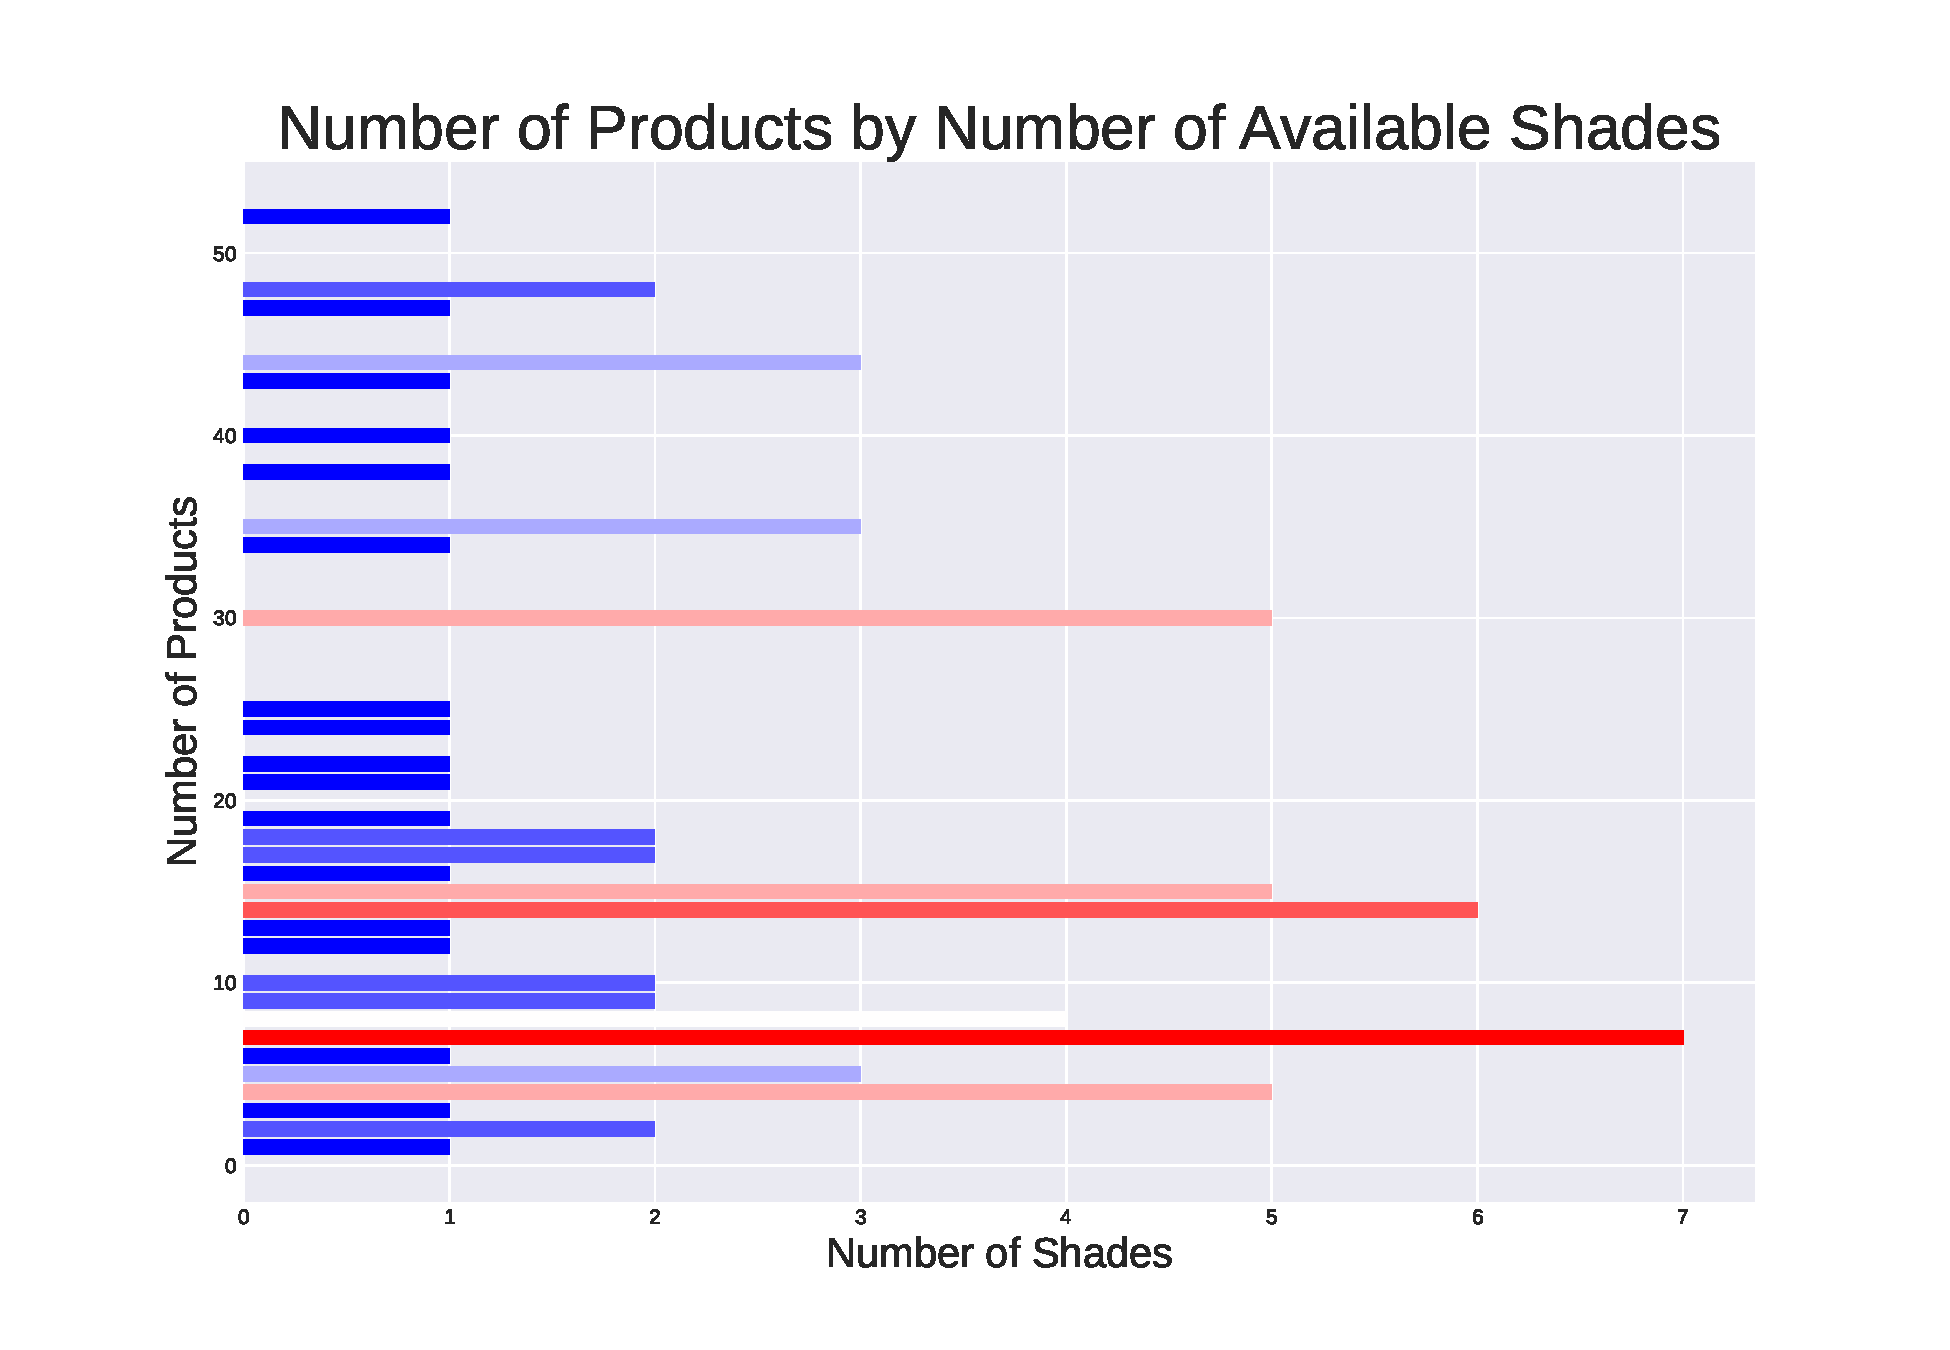
\includegraphics[scale=0.4]{../images/India-graphs/TotalProductsByShades.pdf}
        \caption{Total Products Grouped by Shades - India}
        \label{Products_by_Shades_ind}
    \end{figure}

    \newgeometry{left=2cm,right=2cm, top=1cm, bottom=1.5cm}

    \begin{landscape}
        \begin{figure}[htbp]
            \centering
            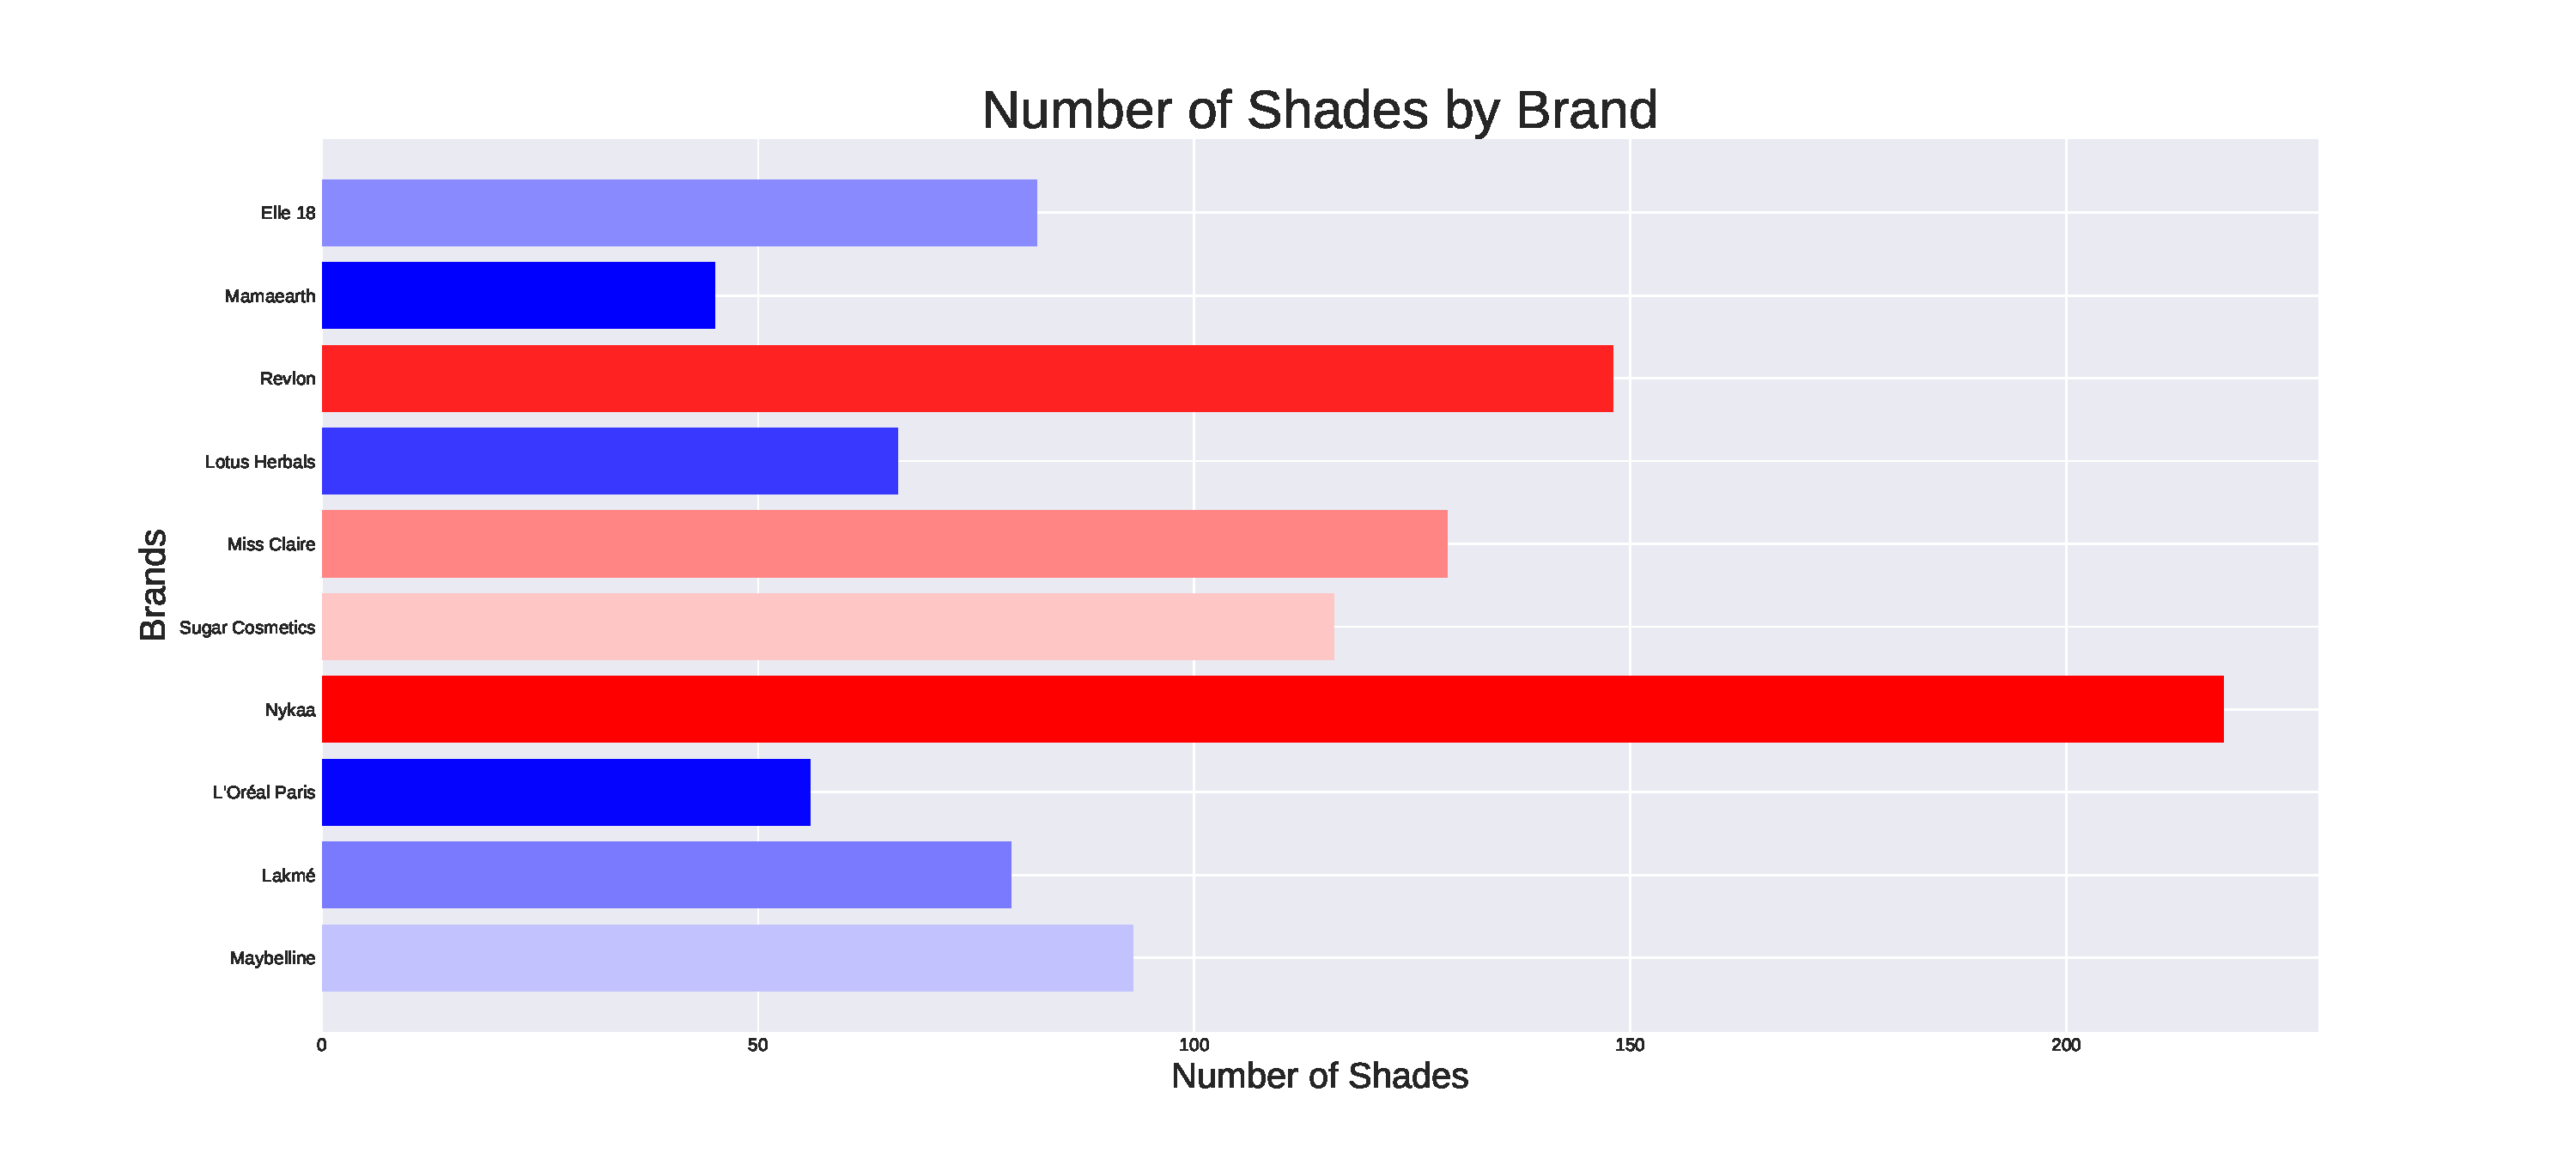
\includegraphics[scale=0.55]{../images/India-graphs/TotalShadesByBrand.pdf}
            \caption{Total Shades Grouped by Brands - India}
            \label{Shades_by_Brand_ind}
        \end{figure}
    \end{landscape}

    \begin{landscape}
        \begin{figure}[htbp]
            \centering
            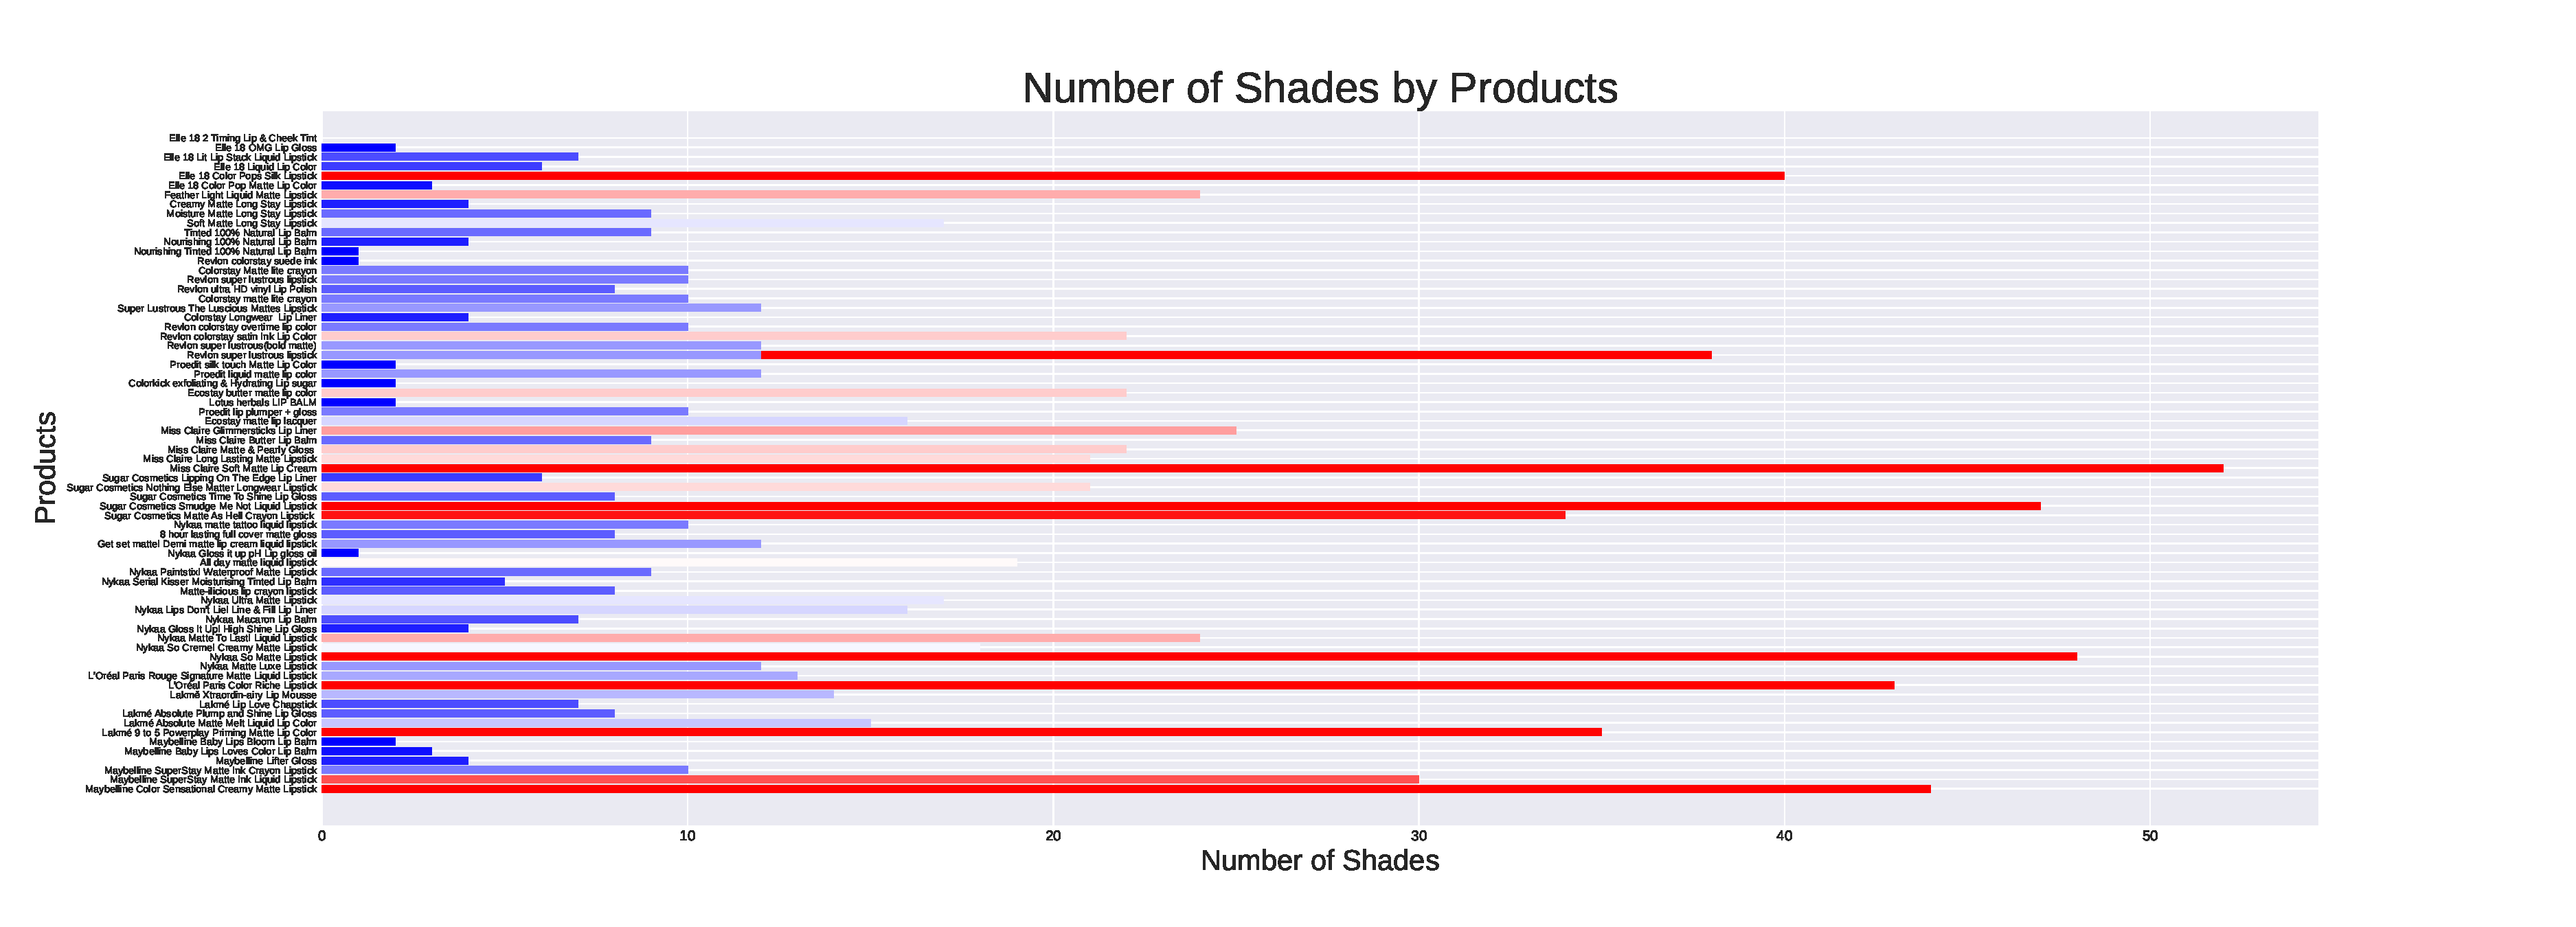
\includegraphics[scale=0.49]{../images/India-graphs/TotalShadesByProduct.pdf}
            \caption{Total Shades Grouped by Product - India}
            \label{Shades_by_Product_ind}
        \end{figure}
    \end{landscape}

    \begin{figure}[htbp]
        \centering
        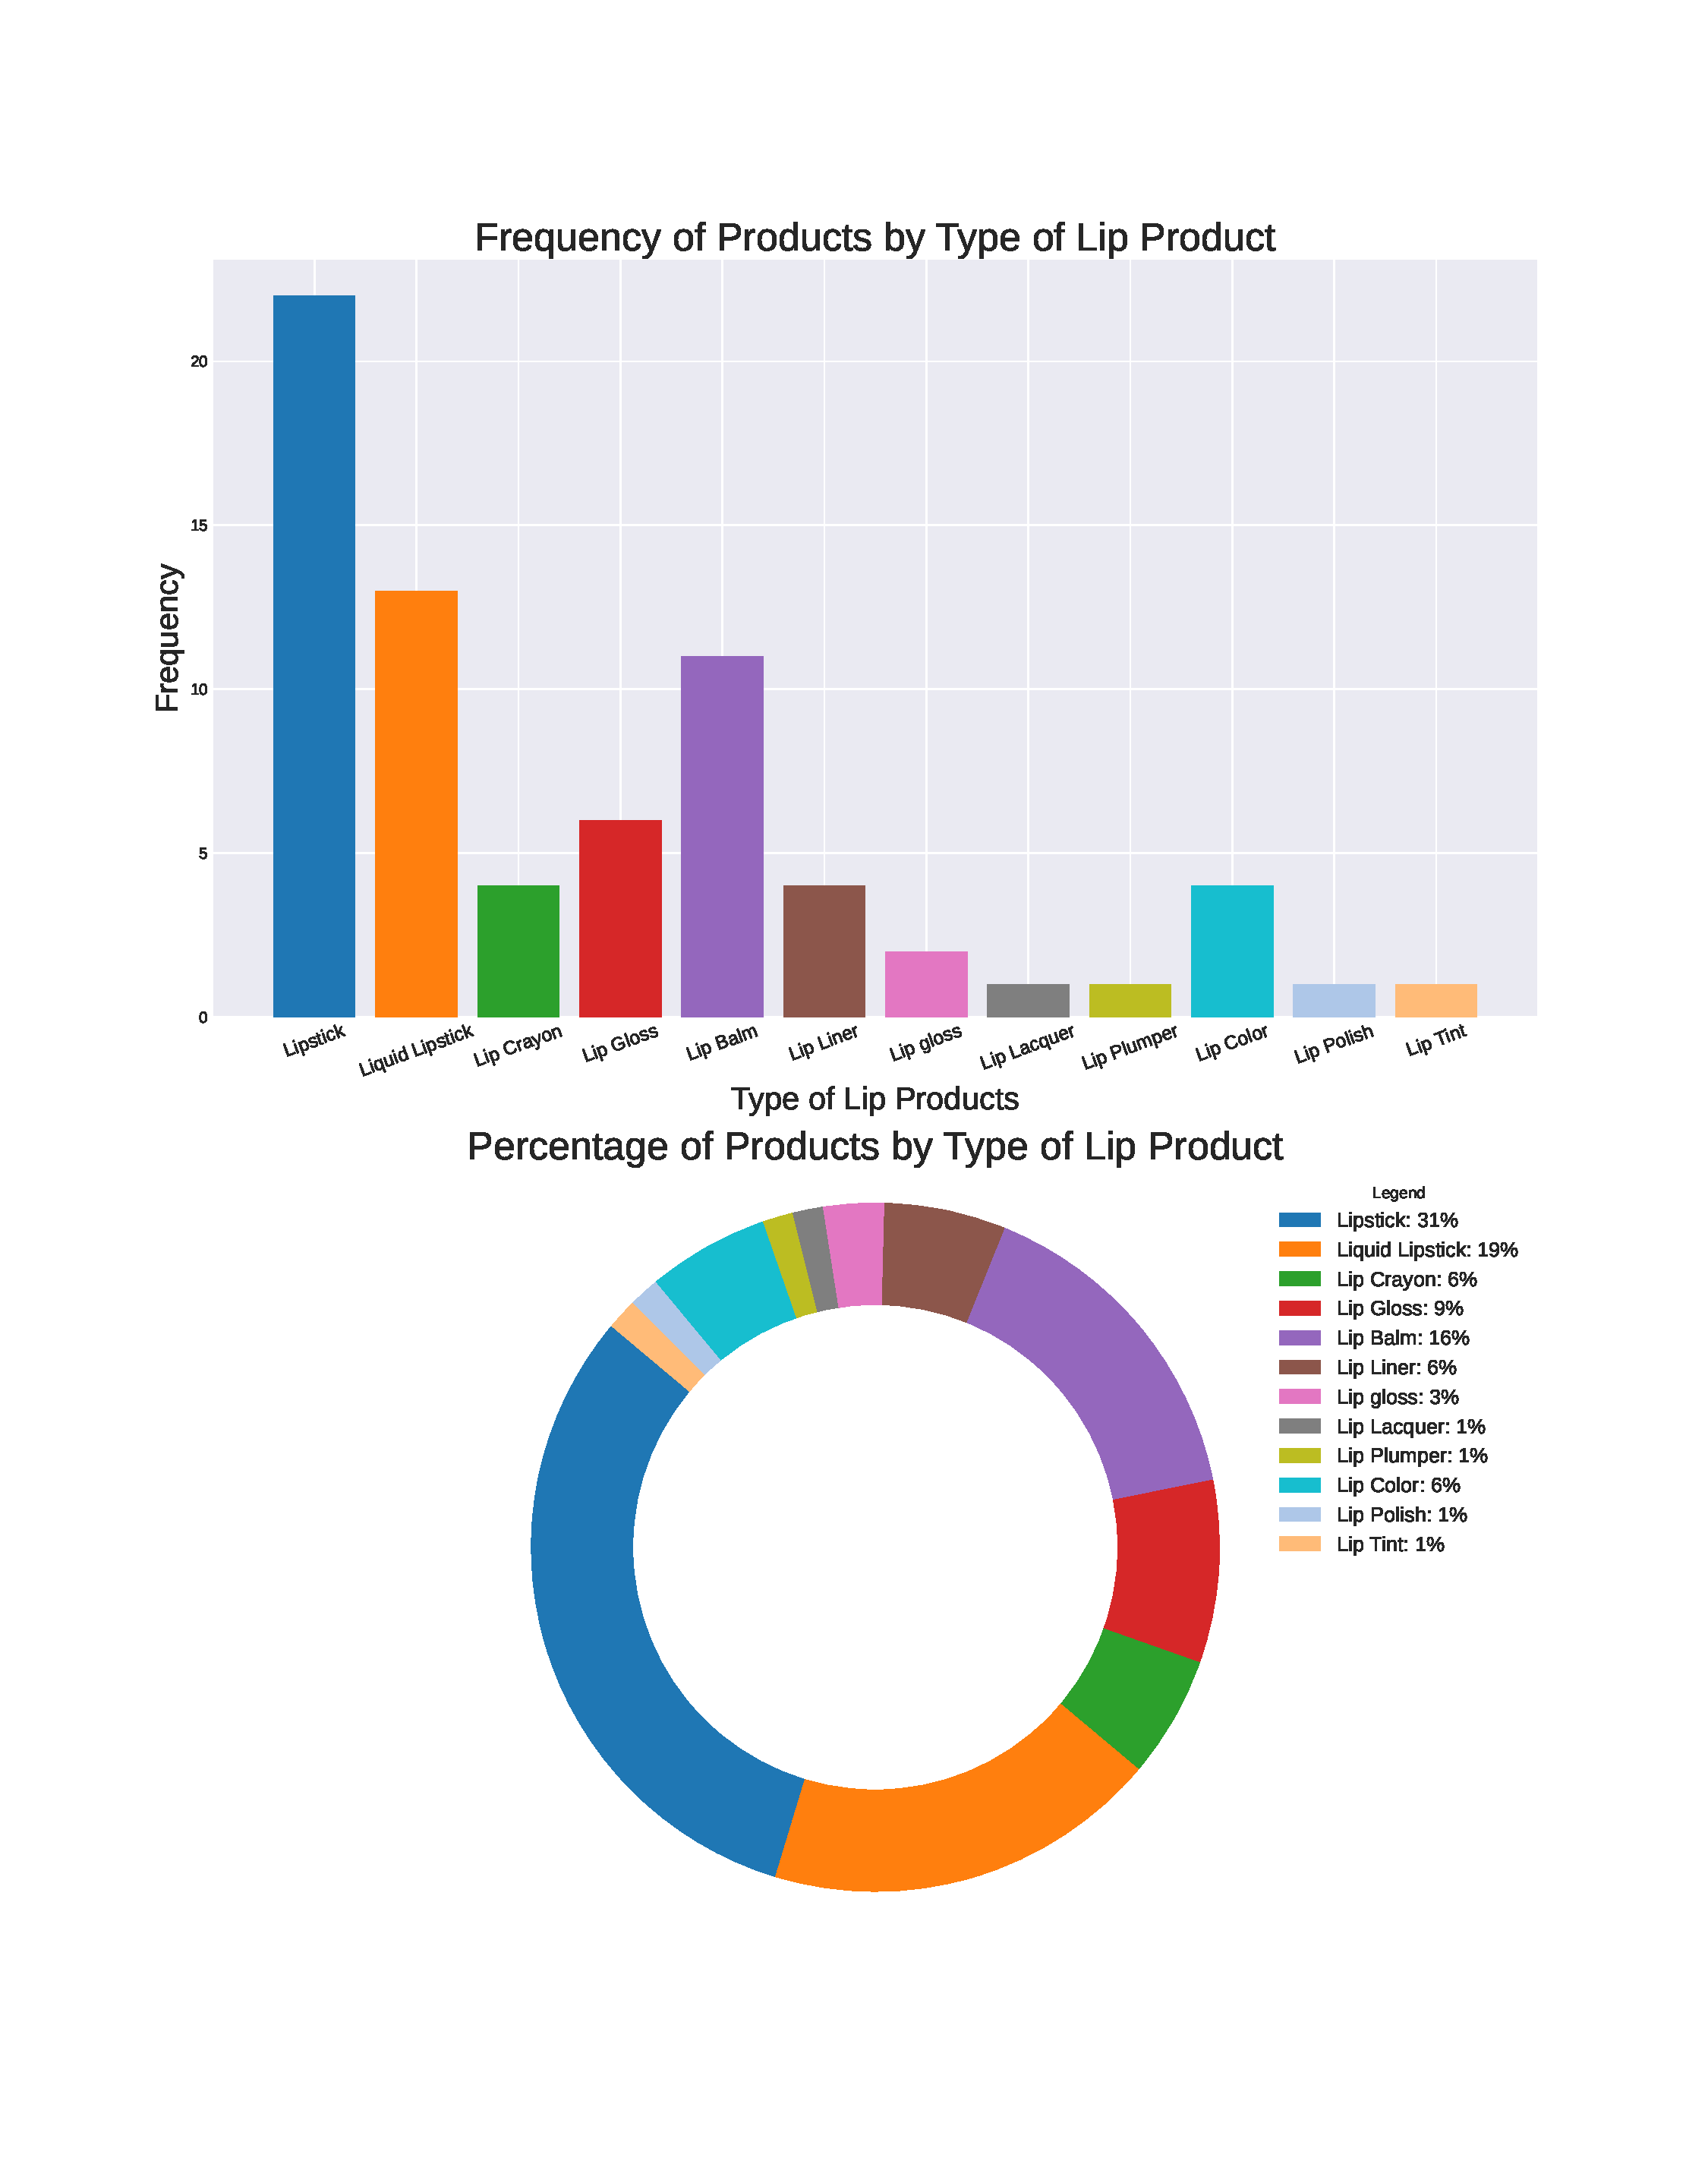
\includegraphics[scale=0.46]{../images/India-graphs/TotalProductsbyType.pdf}
        \caption{Total Products Grouped by Type - India}
        \label{Products_by_Type_ind}
    \end{figure}

    \begin{figure}[htbp]
        \centering
        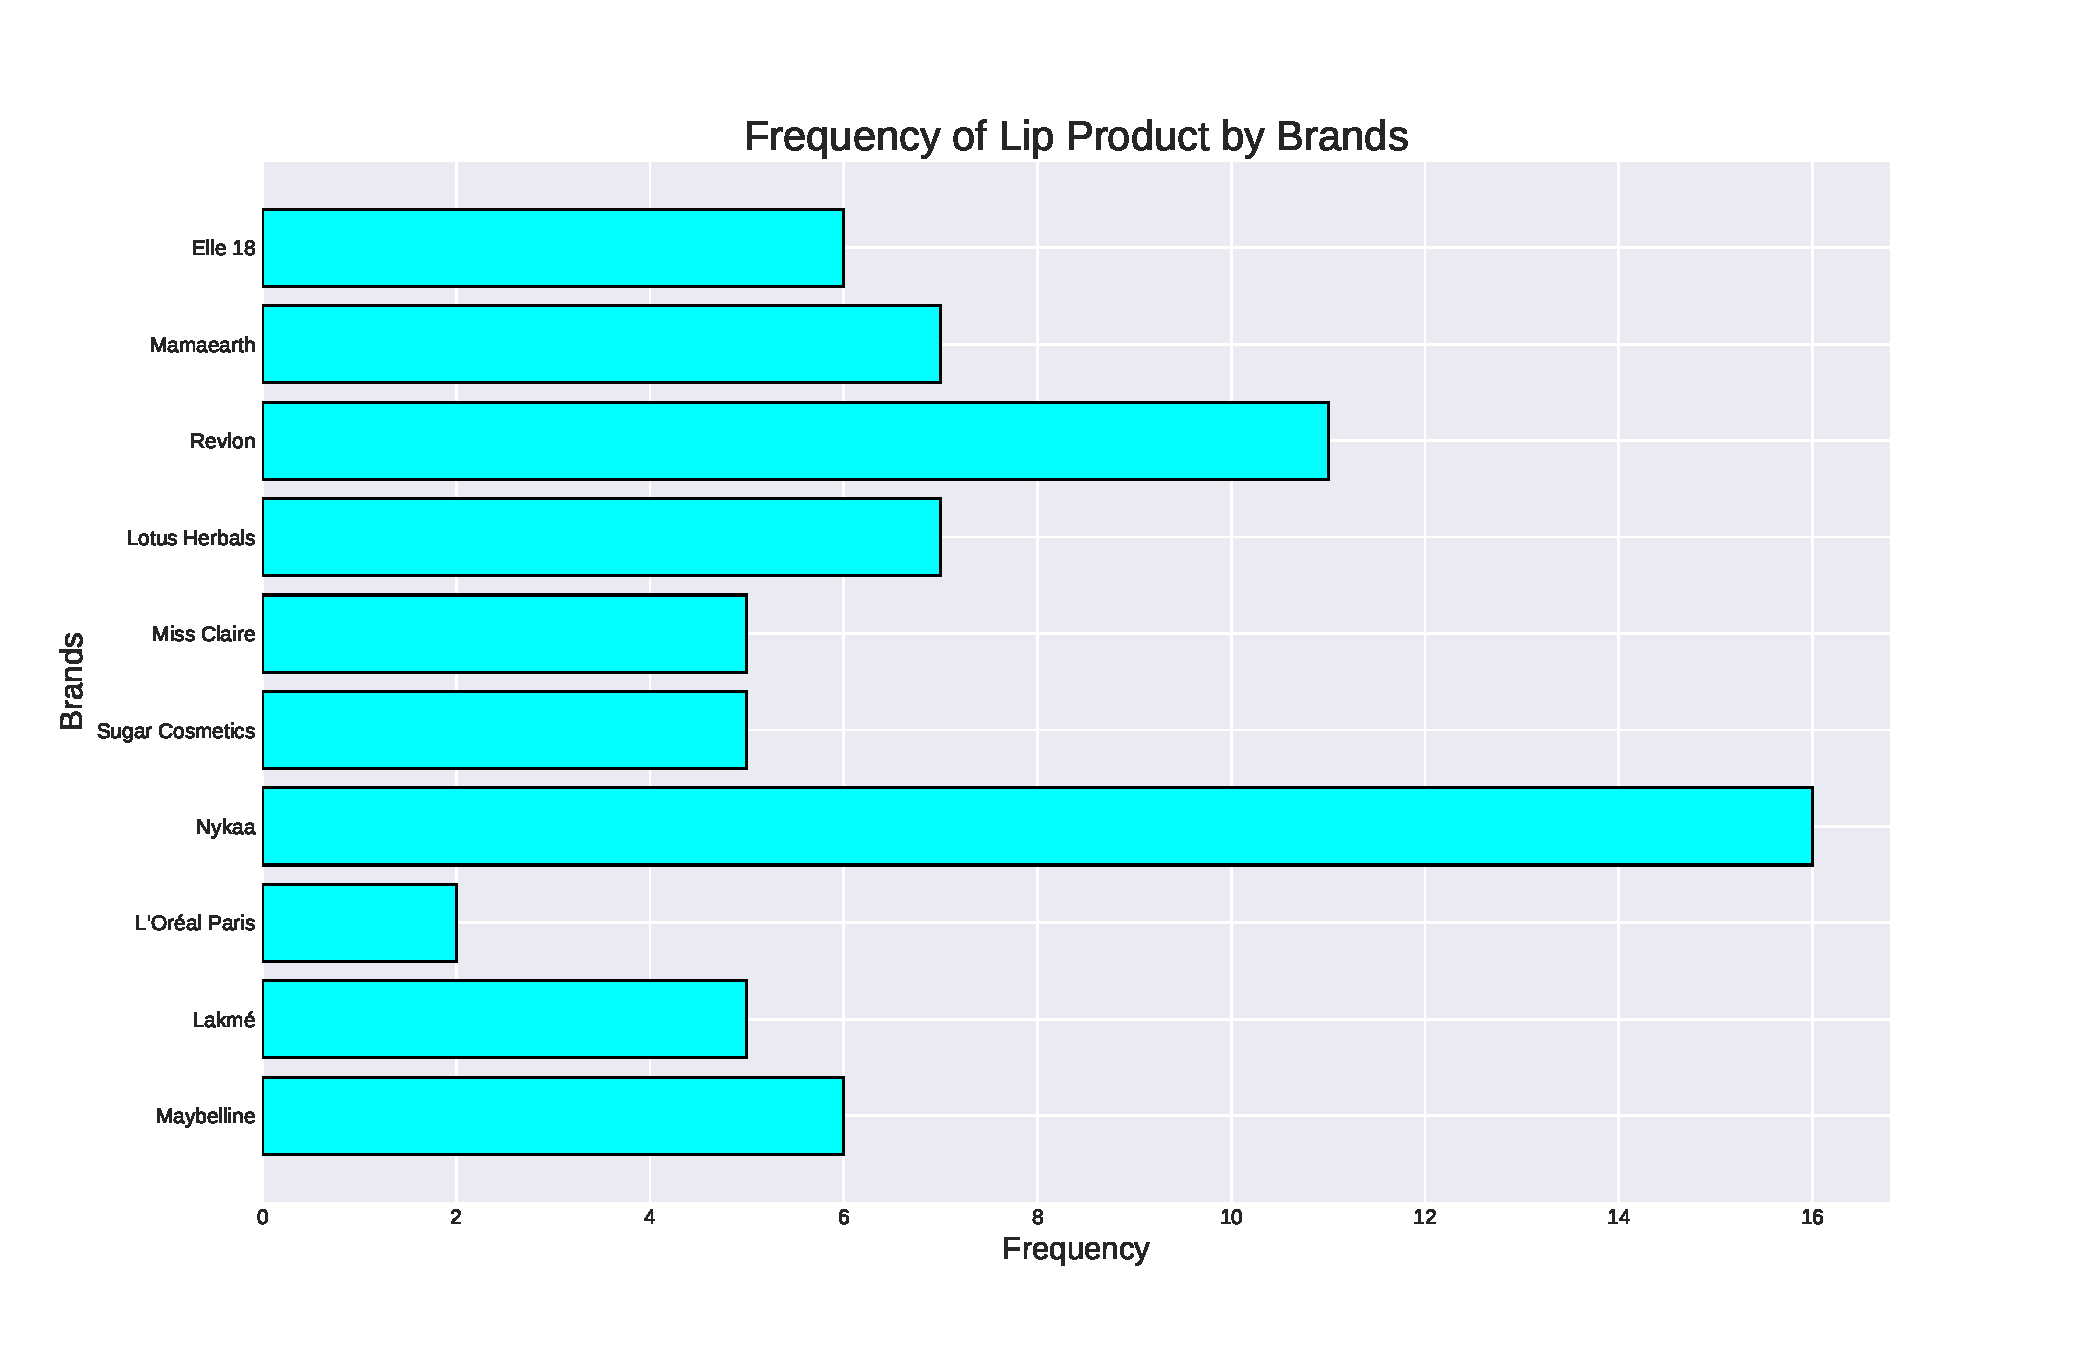
\includegraphics[scale=0.5]{../images/India-graphs/Brand_Frequency.pdf}
        \caption{Frequency of Products by Brands - India}
        \label{Products_by_Brands_ind}
    \end{figure}

    \begin{figure}[htbp]
        \centering
        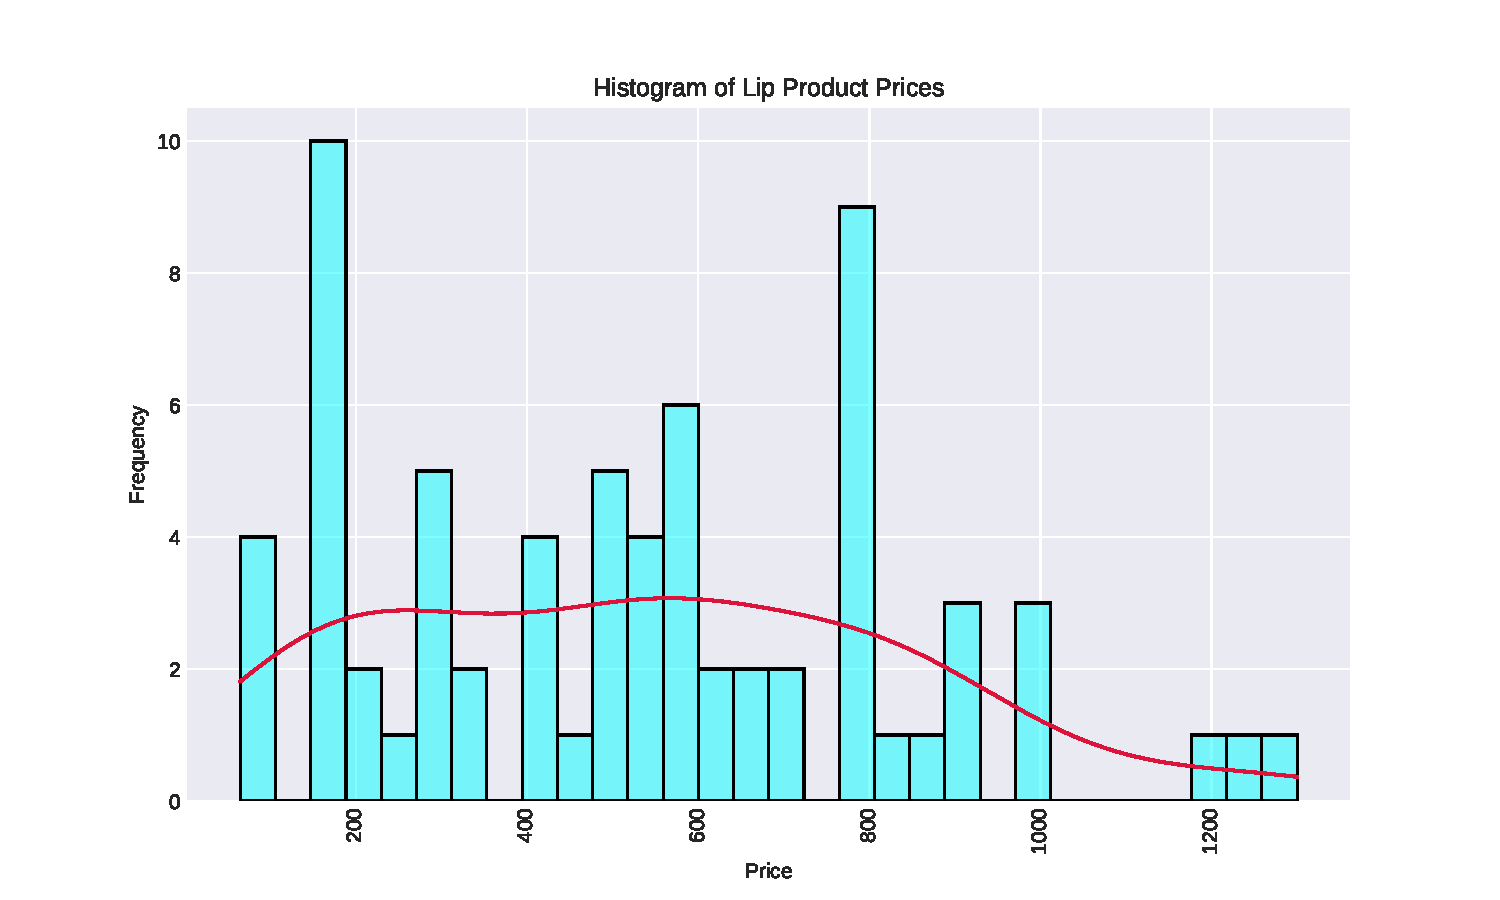
\includegraphics[scale=0.6]{../images/India-graphs/KDE_Prices.pdf}
        \caption{Product - Price Distribution - with KDE - India}
        \label{KDE_Prices_ind}
    \end{figure}

    \begin{figure}[htbp]
        \centering
        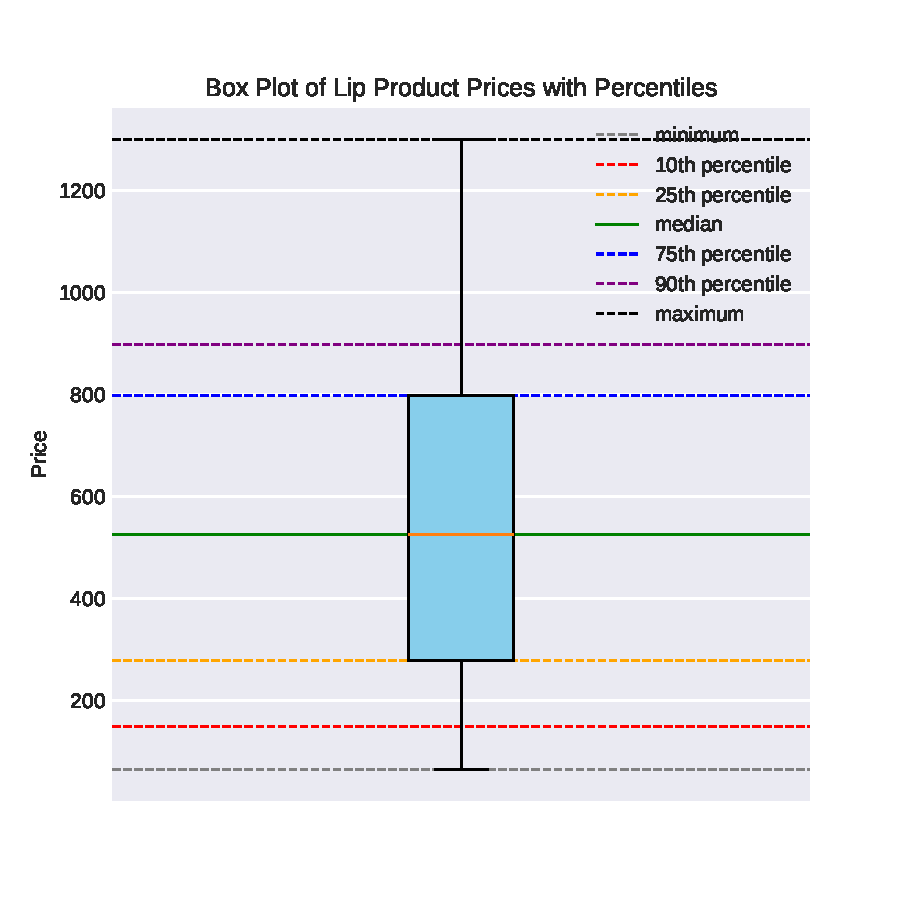
\includegraphics[scale=0.6]{../images/India-graphs/Box_Prices.pdf}
        \caption{Product - Price Distribution - BoxPlot - India}
        \label{Box_Prices_ind}
    \end{figure}

    \begin{figure}[htbp]
        \centering
        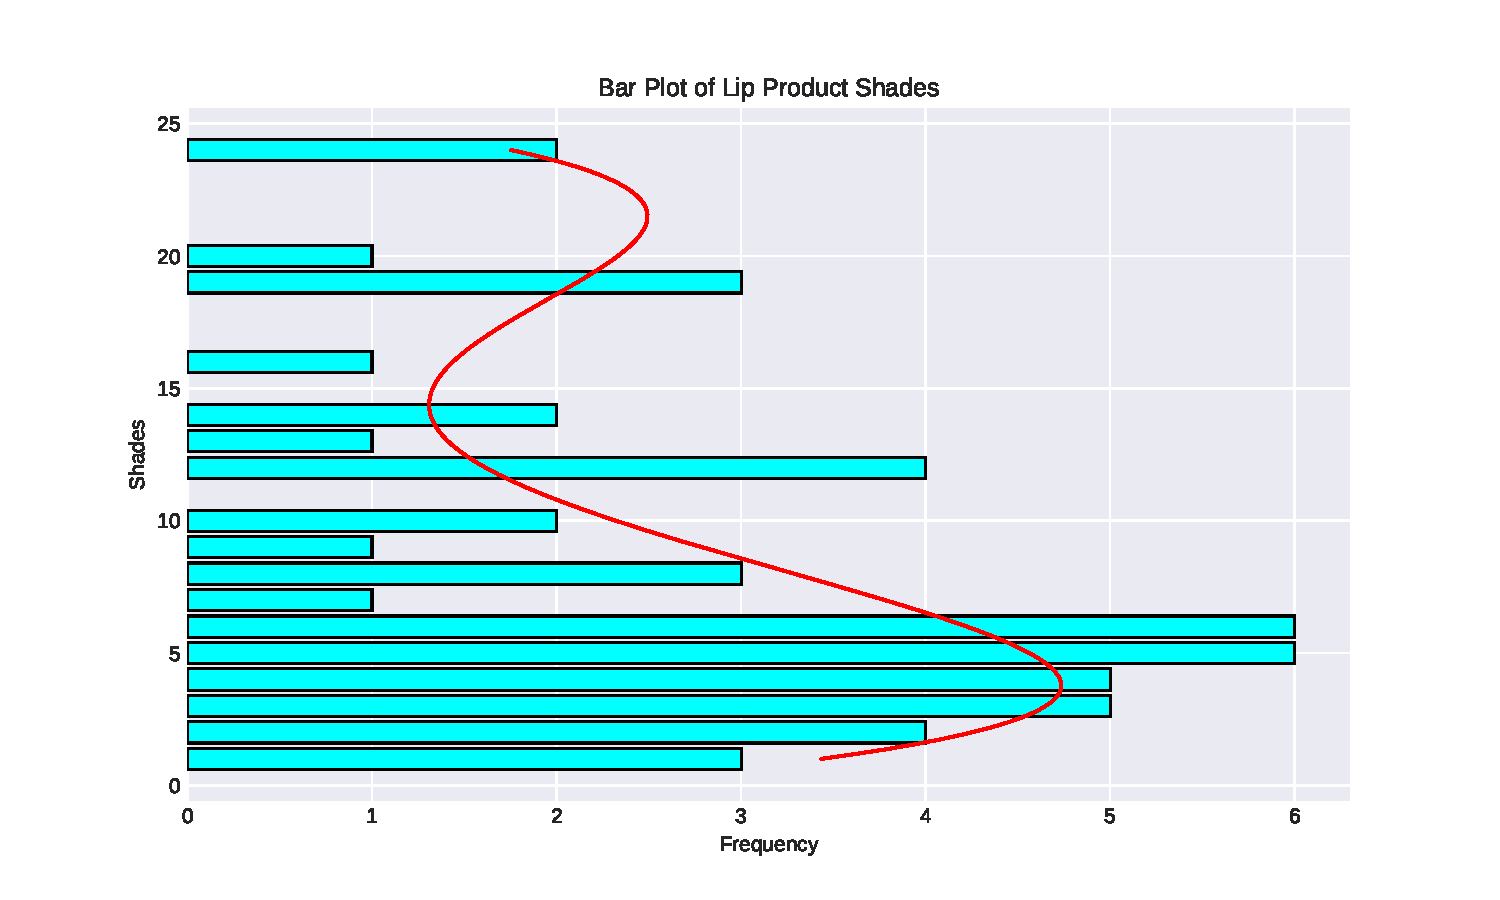
\includegraphics[scale=0.6]{../images/Indonesia-graphs/KDE_Shades.pdf}
        \caption{Product - Shades Distribution - with KDE - India}
        \label{KDE_Shades_ind}
    \end{figure}
    \restoregeometry

\end{center}
\restoregeometry

\section{Survey}

\subsection{Objective}
The primary objective of this study is to ascertain the relative popularity and consumer perceptions of Indian lip product brands among students from diverse backgrounds.

\subsection{Methodology}
A Google Form survey was designed and distributed among students from various educational institutions, ensuring a mix of backgrounds and demographics. The survey included questions related to brand awareness,  satisfaction levels, and factors influencing brand choice.

\subsection{Sample Description}
The survey targeted students aged 17-20 (first and second year college students), encompassing undergraduate levels across different fields of study. The sample size was n=60, with a balanced representation of genders and socio-economic backgrounds. With such a low sample size, there maybe errors and misleading results but the data can be used to get a general idea of the market.

\subsection{Key Findings}
\begin{itemize}
    \item \textbf{Brand Awareness}: Maybelline and Lakmé emerged as the most recognized brands, with 83\% and 87\% awareness respectively, while Revlon got the lowest recognition with merely 35\% awareness.

    \item \textbf{Satisfaction Levels}: In terms of satisfaction, Maybelline scored the highest, with average rating of 77\%  satisfaction with their products. Lakmé followed suit, with a satisfaction rate of 71\%.

    \item \textbf{Most Popular}: Lakmé and Maybelline were the most popular brands, with 47\% and 43\% of respondents respectively having used their products.
\end{itemize}

\subsection{Conclusion}
The survey highlights Maybelline and Lakmé as the most recognized and popular Indian lip product brands among college students. Maybelline leads in satisfaction, while Revlon trails in awareness. These findings emphasize the significance of brand recognition and consumer satisfaction in shaping preferences among this demographic, providing valuable insights for marketing strategies and product development.

\newgeometry{left=0.5cm, right=0.5cm, top=1cm, bottom=2cm}
\begin{center}
    \subsection{Visual Analysis}
\end{center}

\begin{figure}[htbp]
    \centering
    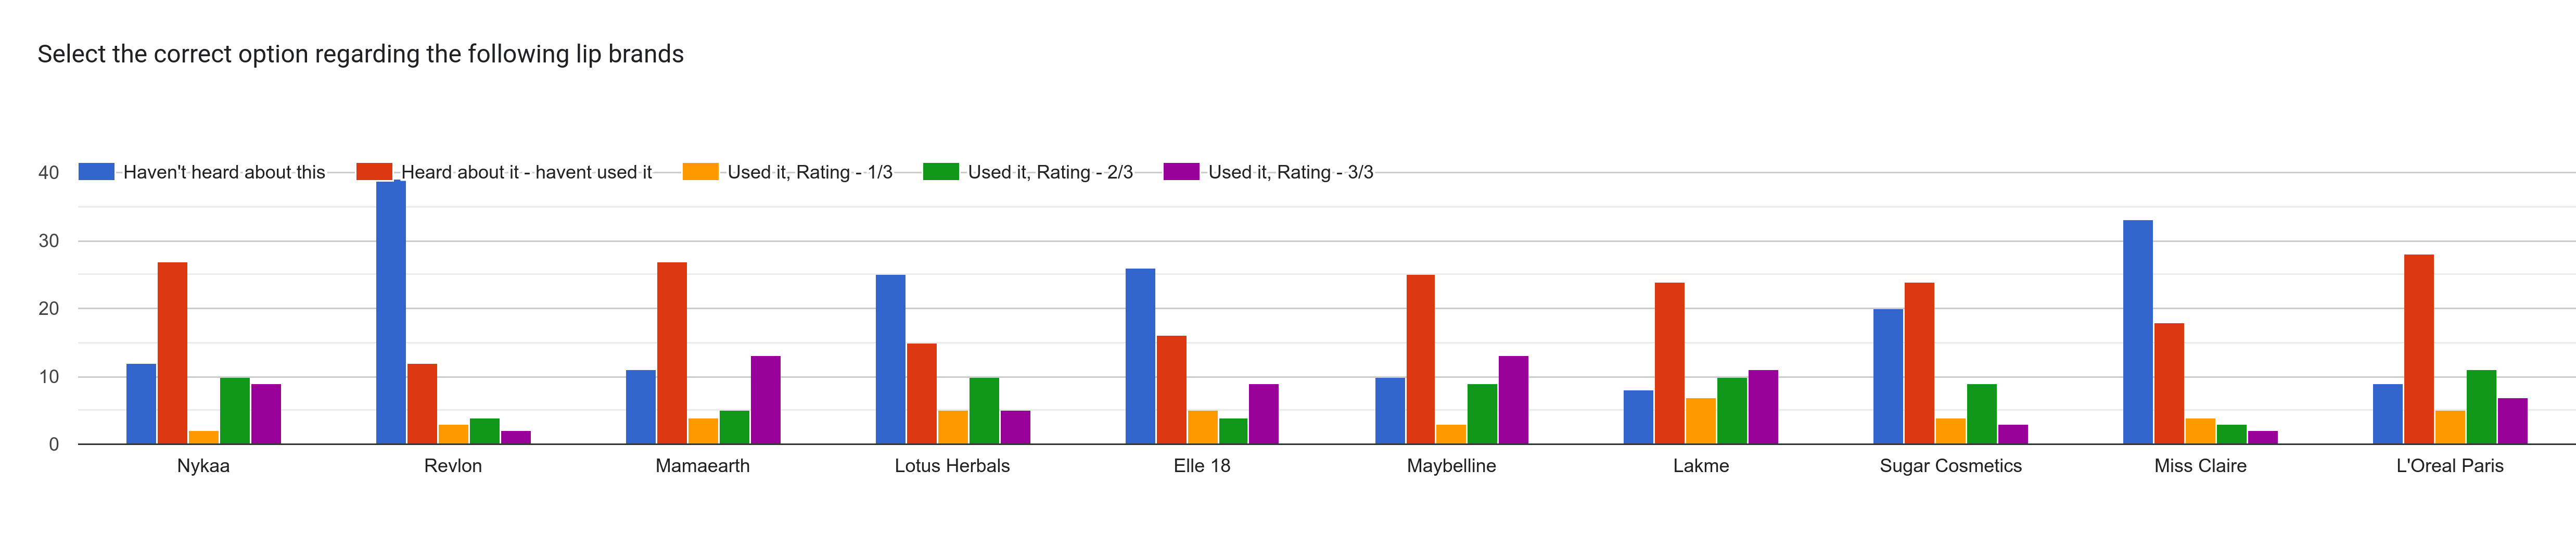
\includegraphics[scale=0.114]{../images/survey-graphs/fromgoogle.png}
\end{figure}

\begin{figure}[htbp]
    \centering
    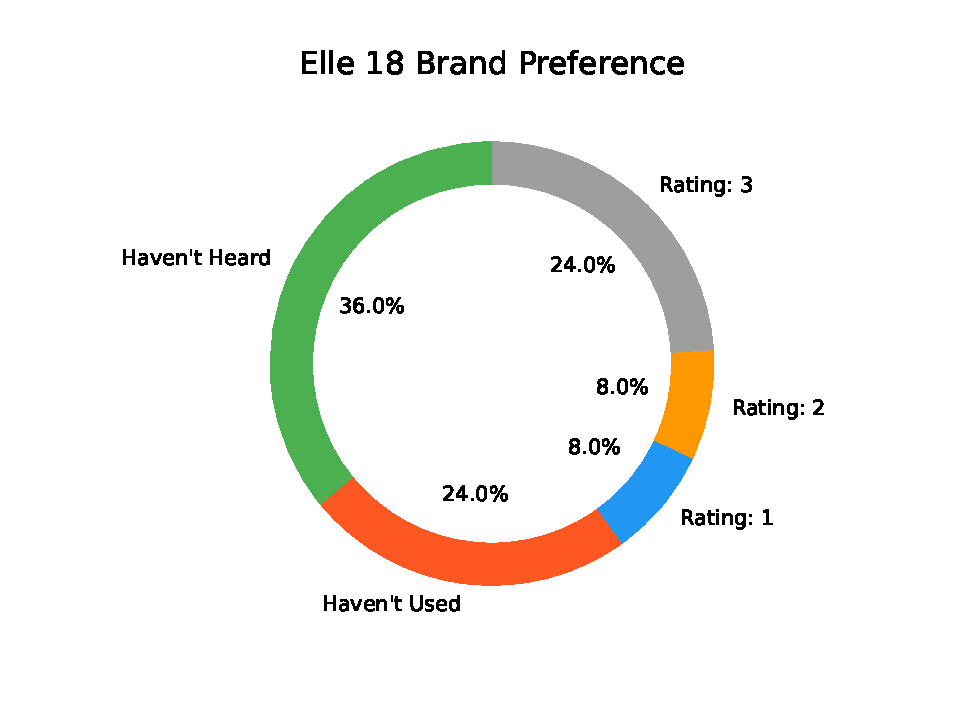
\includegraphics[scale=0.6]{../images/survey-graphs/Elle 18-brand-preference.pdf}
    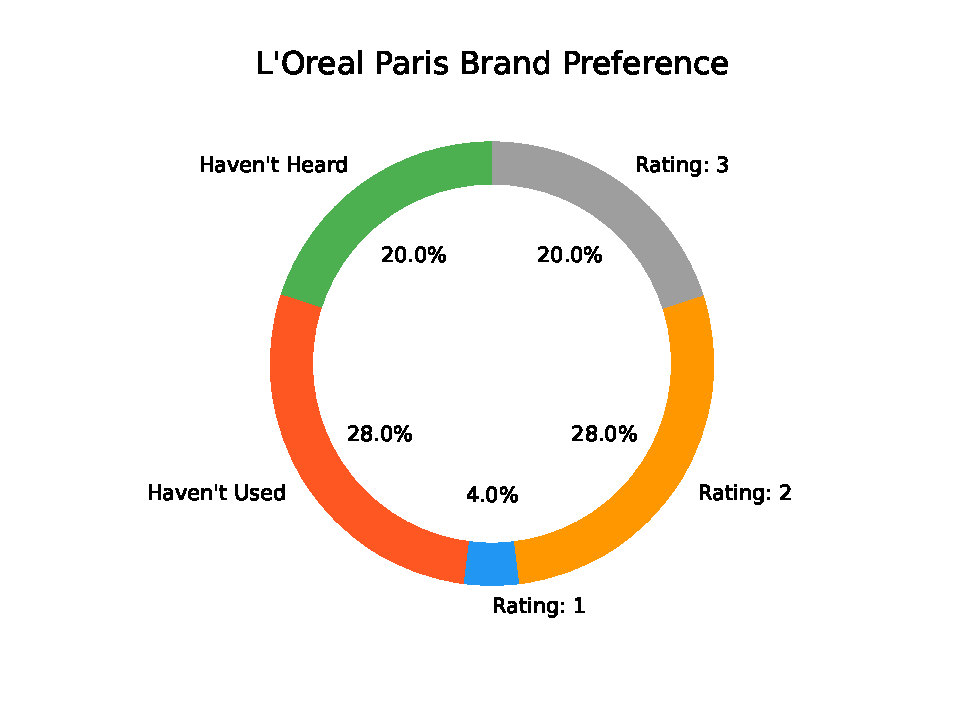
\includegraphics[scale=0.6]{../images/survey-graphs/L'Oreal Paris-brand-preference.pdf}
\end{figure}


\begin{figure}[htbp]
    \centering
    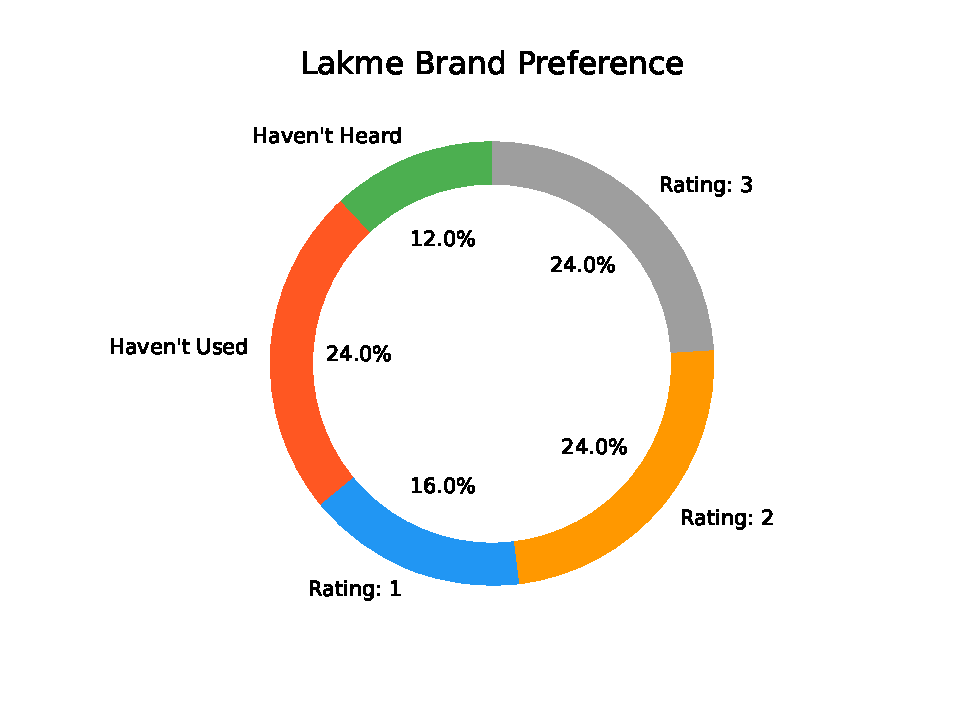
\includegraphics[scale=0.6]{../images/survey-graphs/Lakme-brand-preference.pdf}
    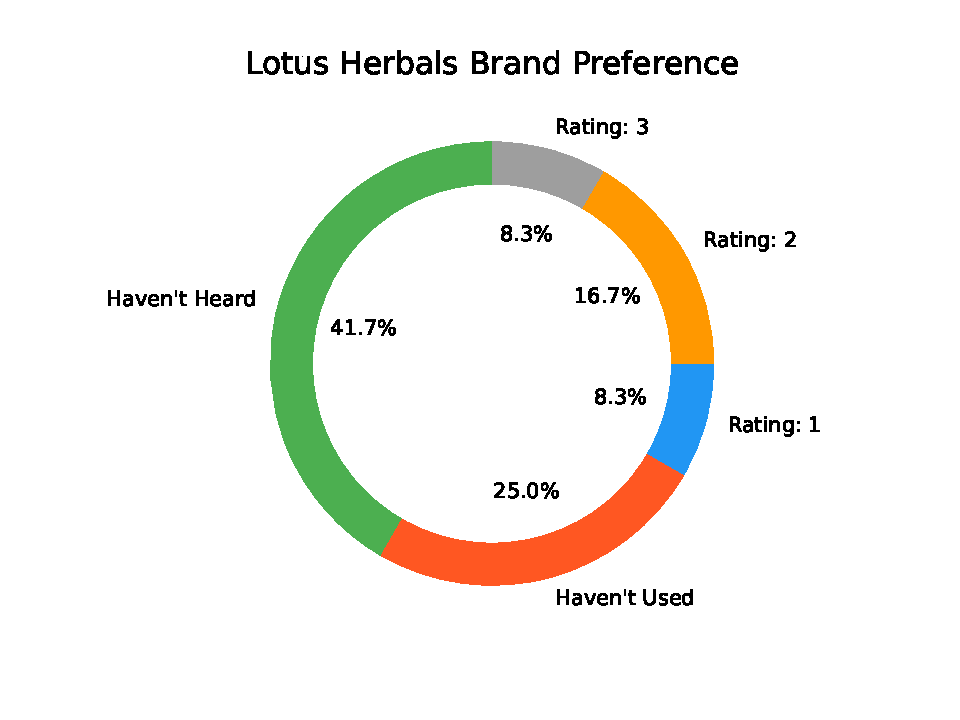
\includegraphics[scale=0.6]{../images/survey-graphs/Lotus Herbals-brand-preference.pdf}
\end{figure}


\begin{figure}[htbp]
    \centering
    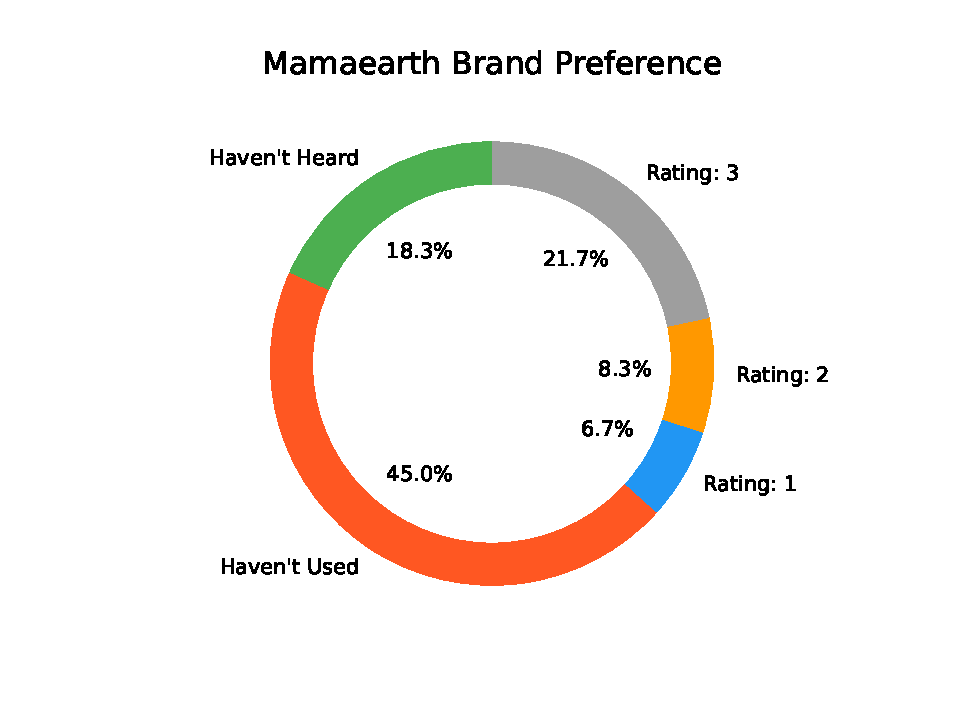
\includegraphics[scale=0.6]{../images/survey-graphs/Mamaearth-brand-preference.pdf}
    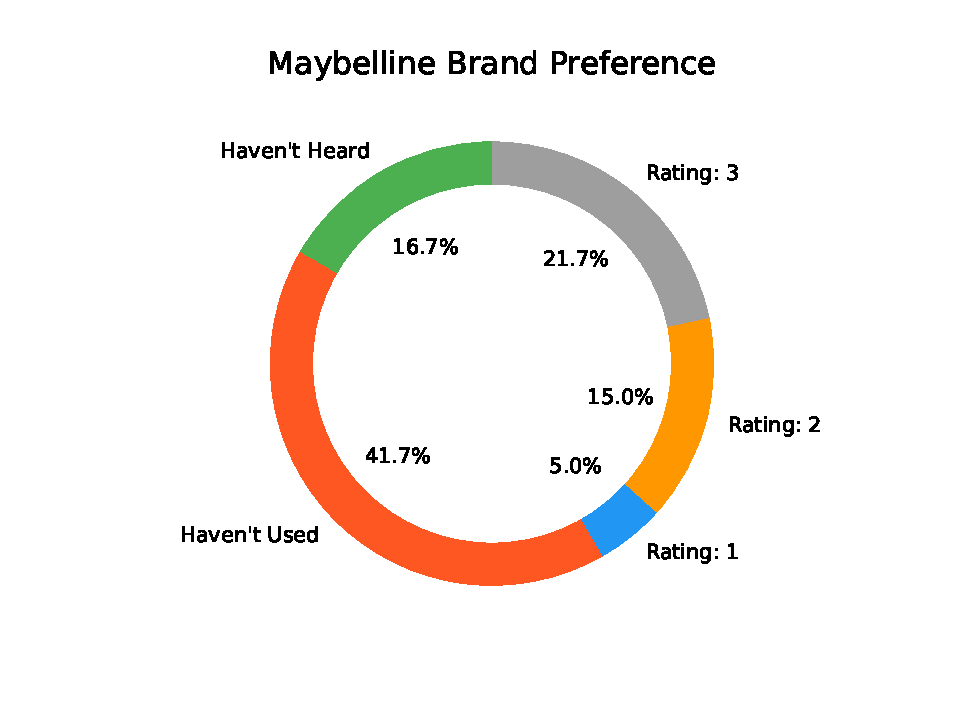
\includegraphics[scale=0.6]{../images/survey-graphs/Maybelline-brand-preference.pdf}
\end{figure}


\begin{figure}[htbp]
    \centering
    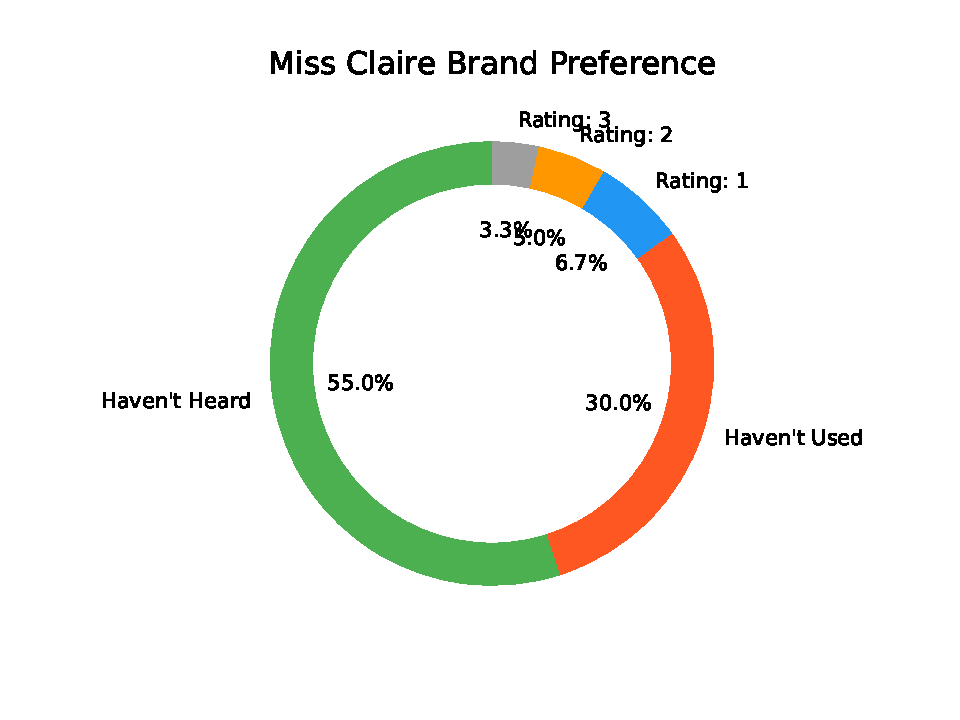
\includegraphics[scale=0.6]{../images/survey-graphs/Miss Claire-brand-preference.pdf}
    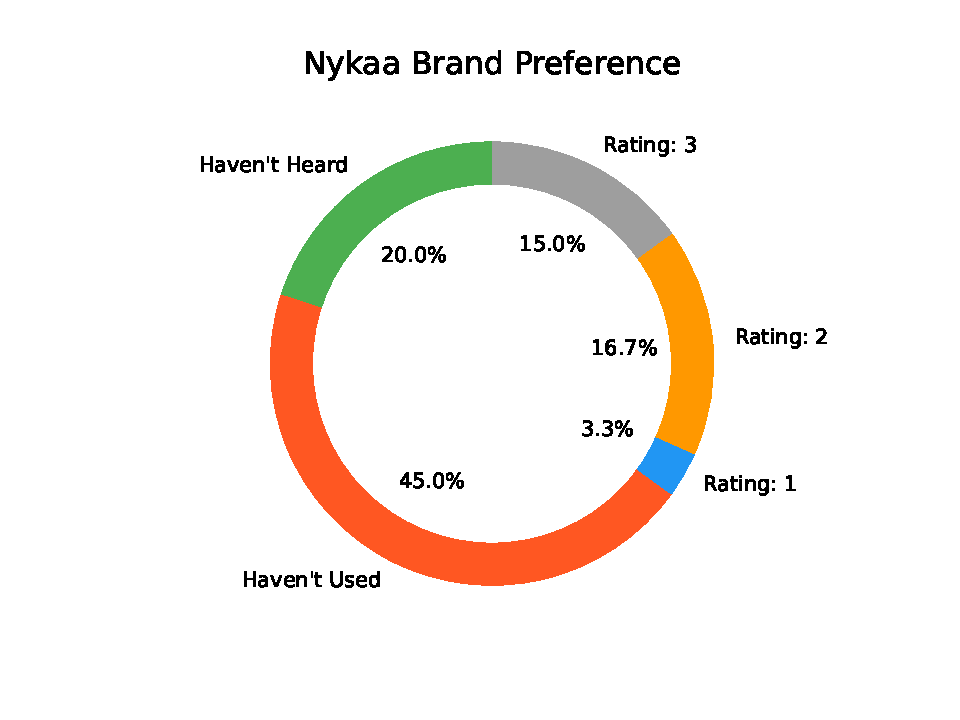
\includegraphics[scale=0.6]{../images/survey-graphs/Nykaa-brand-preference.pdf}
\end{figure}


\begin{figure}[htbp]
    \centering
    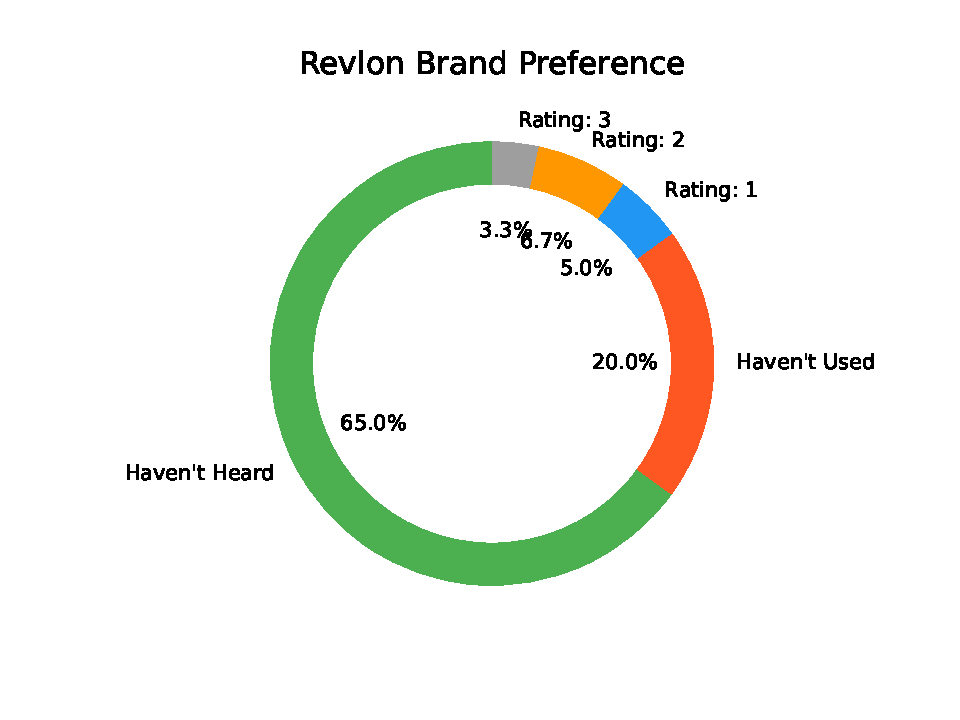
\includegraphics[scale=0.6]{../images/survey-graphs/Revlon-brand-preference.pdf}
    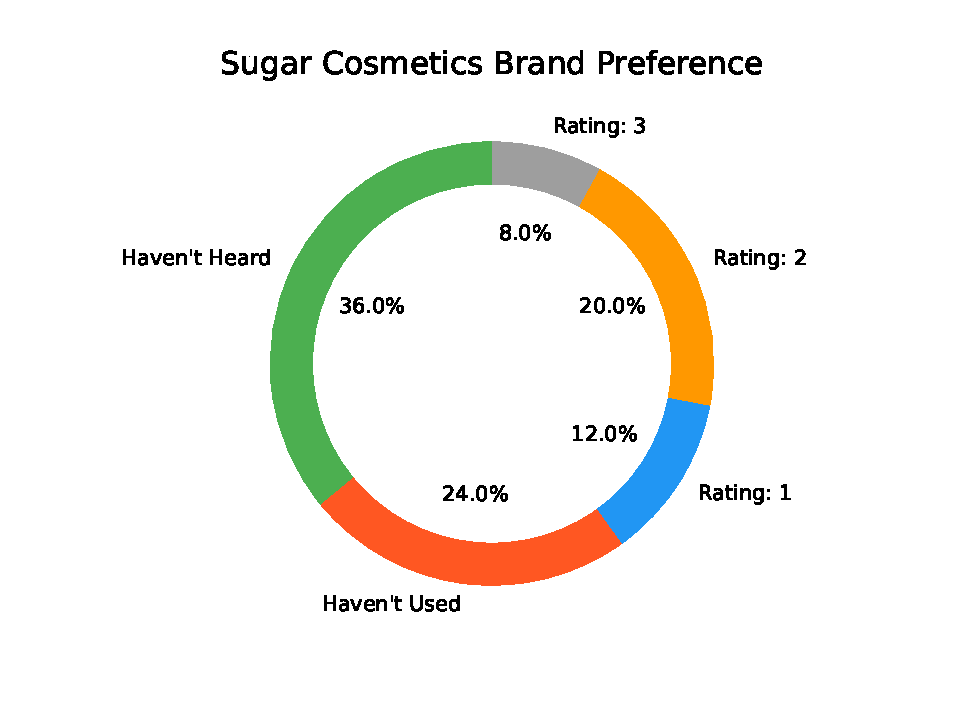
\includegraphics[scale=0.6]{../images/survey-graphs/Sugar Cosmetics-brand-preference.pdf}
\end{figure}


\restoregeometry


\section{Inference}

\subsection{Indonesia}
Most of the products are present in the price range of 15000 to 175000 Indonesian Rupiah, which roughly translates to INR 80 - 900. Some of the products lie outside this range and can be seen as occasional peaks in the bar plot. The maximum price of any product is Ru 711636 and the minimum is Ru 15765. The mean price of all products is Ru 104456 (INR 544) and the median is Ru 84000. The data also shows a standard deviation of around 105480. \\

\noindent The number of shades per product varies from 1 to 24, with the mean being 8.04 and the median being 6. Also, companies like Wardah, Maybelline, Makeover, L'oreal and Implora boast a large number of shades in their products while other companies do not have as much variety. \\

\noindent Both variables have relatively high standard deviations compared to their means, indicating wide variability when it comes to prices and shade counts around their respective averages. \\

\noindent Outliers are present in both variables, especially considering the large difference between the 75th percentile and the maximum values for both price and shades. \\

\noindent Most of the lip products produced by these brands fall under the 'liquid' category, as evident from the donut chart. It accounts for 72 percent of the total products. From the remaining, 24 percent are 'stick' type and solid and crayon account for 2 percent each. \\

\noindent Also, most companies only have one product present in the data, with some exceptions being Emina, L'oreal, Luxcrime, Madame Gie, Makeover, Maybelline and Wardah which have 2 or more products each. Emina, Wardah and Maybelline form the most popular brands in Indonesia closely followed by Madame Gie and L'oreal. \\

\subsection{India}
\noindent Most of the products were observed to lie in the price range of Rs. 200 to Rs. 800. The median of prices was found to be Rs. 525, while the number of shades vary from 1 to 52, with the median being 10. Outliers exist in both datasets.\\

\noindent The standard deviation for shades is around 12.72, indicating a moderate amount of variability in the number of shades. For prices, the standard deviation is approximately Rs. 305.88, suggesting a lot of variability in the prices of lipsticks. A wide range of shades are available for people to choose from and there are many affordable options as well as expensive.\\

\noindent Lipstick and Liquid Lipstick Dominate: Lipstick and liquid lipstick are the most prevalent types of lip products, together accounting for nearly 50\% of the total distribution. This suggests that these two forms are likely the most popular choices among consumers.\\

\noindent The data shows a diverse range of lip product types, including lip balm, lip gloss, lip liner, lip crayon, etc. This indicates that consumers have a variety of options to choose from based on their preferences and needs, such as hydration, color intensity, or longevity.\\

\noindent Traditional lip products like lipstick, lip gloss, and lip balm seem to be more popular compared to newer or specialized forms like lip lacquer, lip plumper, or lip polish. This suggests that consumers may have established preferences for classic lip product formulations.\\

\noindent While some products like lipstick and lip gloss are mainstream and widely used, there are also niche products like lip lacquer, lip plumper, and lip tint, each representing a smaller portion of the market. These niche products may cater to specific consumer preferences or trends.\\

\noindent The presence of newer product types like lip lacquer and lip plumper, although in smaller proportions, suggests that there is ongoing innovation in the lip product industry to introduce new formulations and meet evolving consumer demands.\\

\noindent Nykaa emerges as the leading brand with the highest frequency, constituting approximately 22.86\% of the total distribution. This indicates that Nykaa holds a significant market share and is likely a popular choice among consumers.\\

\noindent Indian brands such as Nykaa, Lakmé, Sugar Cosmetics, Miss Claire, Lotus Herbals, Mamaearth, and Elle 18 collectively make up a significant portion of the market, representing approximately 65.71\% of the total distribution. This highlights the growing prominence and competitiveness of Indian brands in the lipstick market.\\

\noindent Established international brands like Maybelline, L'Oréal Paris, and Revlon also have a notable presence.\\

\noindent Brands like Nykaa, Elle 18, and Mamaearth, known for offering affordable and budget-friendly products, have a considerable share of the market. This suggests that consumers are inclined towards brands that offer good quality at competitive prices.\\

\noindent The presence of multiple brands in the market provides consumers with a wide range of options to choose from, allowing them to select products based on factors such as brand reputation, product quality, price, and availability.\\

\noindent Also, while Nykaa holds the highest frequency, the market is not overly concentrated at one point, as there is a distribution of market share among several brands. This indicates healthy competition within the lipstick market, fostering innovation and diverse offerings for consumers.

\section{Comparative Study}

\begin{itemize}
    \item \textbf{Prices}: Indonesia has a broader price range, with products ranging from Rp 15,765 to Rp 711,636. The median price is Rp 84,000. In contrast, prices in India are generally lower, ranging from Rs. 200 to Rs. 800, with a median price of Rs. 525. Indonesia has a higher maximum price and wider price range compared to India.
    \item \textbf{Shade Variety}: India offers a wider range of shades per product, with the number of shades varying from 1 to 52 and a median of 10 shades. In comparison, Indonesia has a lower average number of shades per product, ranging from 1 to 24, with an average of 8.04 shades. India provides a more diverse selection of shades for consumers to choose from.
    \item \textbf{Price Variability}: Indonesia has a higher standard deviation for prices (Rp 105,480) compared to India (Rs. 305.88), indicating greater variability in pricing. This suggests that prices in Indonesia fluctuate more widely around the mean price, potentially influenced by factors such as brand positioning, product features, and market demand.
    \item \textbf{Brands}: India has a larger presence of domestic brands, with Nykaa leading the market in terms of frequency (22.86\%). Indian brands collectively hold a significant share (65.71\%). International brands like Maybelline, L'Oréal Paris, and Revlon also have a notable presence. In comparison, Indonesia has a more even distribution of brands, with Emina, Wardah, Maybelline, L'Oréal, and Makeover having multiple products, while many brands have only one product.
\end{itemize}

% Bibliography
\newpage
\bibliographystyle{unsrt}
\bibliography{references}
\addcontentsline{toc}{section}{\refname}

\newpage
\newgeometry{left=1cm,right=1cm}
\begin{center}
    \section*{Contributions}
\end{center}
\begin{table}[htbp]
    \centering
    \caption{Contributions of the authors}
    \label{tab:Table_Contri}
    \begin{tabular}{|c|c|c|c|c|c|}
        \hline
        \textbf{\thead{Name}} & \textbf{\thead{Roll No.}} & \textbf{\thead{Contribution \\ in Report Writing}} & \textbf{\thead{Contribution \\ in Analysis}} & \textbf{\thead{Details of use \\ of web resources/\\Codes/AI tools, etc.}} & \textbf{\thead{Overall \\ Contribution \\ to work done}} \\ \hline
        Arka Mukhopadhyay & B23120 & Remaining & \begin{tabular}{@{}c@{}}Grouping products \\ by brands and type \end{tabular} & \begin{tabular}{@{}c@{}} CSV to LaTeX \\ table converters \end{tabular} & 16.8 \\ \hline
        Pranab Ray & B23169 & \begin{tabular}{@{}c@{}}Data Analysis \\ Inference\end{tabular}& \begin{tabular}{@{}c@{}} Remaining \end{tabular} & \begin{tabular}{@{}c@{}}ChatGPT and Gemini \\ to refine writeups \end{tabular} & 16.8 \\ \hline
        Kamal Yadav & B23209 & Data Collection & \begin{tabular}{@{}c@{}}Collecting \\ Indian Data \end{tabular} & - & 16.6 \\ \hline
        Arani Ghosh & B23119 & - & \begin{tabular}{@{}c@{}}KDE and \\ Descriptive Statistics \end{tabular} & \begin{tabular}{@{}c@{}}GitHub Copilot \\ to beautify graphs \end{tabular} & 16.6 \\ \hline
        Ayuj Aryan & B23198 & Data Collection & \begin{tabular}{@{}c@{}}Collecting \\ Indonesian Data \end{tabular} & - & 16.6 \\ \hline
        Kunal Sharma & B23079 & Data Collection & \begin{tabular}{@{}c@{}}Collecting \\ Indian Data \end{tabular} & - & 16.6 \\ \hline
    \end{tabular}
\end{table}
\restoregeometry

\end{document}